\documentclass[]{article}
\usepackage{lmodern}
\usepackage{amssymb,amsmath}
\usepackage{ifxetex,ifluatex}
\usepackage{fixltx2e} % provides \textsubscript
\ifnum 0\ifxetex 1\fi\ifluatex 1\fi=0 % if pdftex
  \usepackage[T1]{fontenc}
  \usepackage[utf8]{inputenc}
\else % if luatex or xelatex
  \ifxetex
    \usepackage{mathspec}
  \else
    \usepackage{fontspec}
  \fi
  \defaultfontfeatures{Ligatures=TeX,Scale=MatchLowercase}
\fi
% use upquote if available, for straight quotes in verbatim environments
\IfFileExists{upquote.sty}{\usepackage{upquote}}{}
% use microtype if available
\IfFileExists{microtype.sty}{%
\usepackage{microtype}
\UseMicrotypeSet[protrusion]{basicmath} % disable protrusion for tt fonts
}{}
\usepackage[margin=1in]{geometry}
\usepackage{hyperref}
\hypersetup{unicode=true,
            pdftitle={Learning pleiotropic signatures to construct a causal map of the human phenome},
            pdfborder={0 0 0},
            breaklinks=true}
\urlstyle{same}  % don't use monospace font for urls
\usepackage{graphicx,grffile}
\makeatletter
\def\maxwidth{\ifdim\Gin@nat@width>\linewidth\linewidth\else\Gin@nat@width\fi}
\def\maxheight{\ifdim\Gin@nat@height>\textheight\textheight\else\Gin@nat@height\fi}
\makeatother
% Scale images if necessary, so that they will not overflow the page
% margins by default, and it is still possible to overwrite the defaults
% using explicit options in \includegraphics[width, height, ...]{}
\setkeys{Gin}{width=\maxwidth,height=\maxheight,keepaspectratio}
\IfFileExists{parskip.sty}{%
\usepackage{parskip}
}{% else
\setlength{\parindent}{0pt}
\setlength{\parskip}{6pt plus 2pt minus 1pt}
}
\setlength{\emergencystretch}{3em}  % prevent overfull lines
\providecommand{\tightlist}{%
  \setlength{\itemsep}{0pt}\setlength{\parskip}{0pt}}
\setcounter{secnumdepth}{0}
% Redefines (sub)paragraphs to behave more like sections
\ifx\paragraph\undefined\else
\let\oldparagraph\paragraph
\renewcommand{\paragraph}[1]{\oldparagraph{#1}\mbox{}}
\fi
\ifx\subparagraph\undefined\else
\let\oldsubparagraph\subparagraph
\renewcommand{\subparagraph}[1]{\oldsubparagraph{#1}\mbox{}}
\fi
\usepackage{amsmath}

%%% Use protect on footnotes to avoid problems with footnotes in titles
\let\rmarkdownfootnote\footnote%
\def\footnote{\protect\rmarkdownfootnote}

%%% Change title format to be more compact
\usepackage{titling}

% Create subtitle command for use in maketitle
\newcommand{\subtitle}[1]{
  \posttitle{
    \begin{center}\large#1\end{center}
    }
}

\setlength{\droptitle}{-2em}
  \title{Learning pleiotropic signatures to construct a causal map of the human
phenome}
  \pretitle{\vspace{\droptitle}\centering\huge}
  \posttitle{\par}
  \author{}
  \preauthor{}\postauthor{}
  \predate{\centering\large\emph}
  \postdate{\par}
  \date{02 August 2017}

\begin{document}
\maketitle

Gibran Hemani\(^1\), Jack Bowden\(^1\), Philip Haycock\(^1\), Jie
Zheng\(^1\), Oliver Davis\(^1\), Peter Flach\(^2\), Tom Gaunt\(^{1,*}\),
George Davey Smith\(^{1,*}\)

\begin{enumerate}
\def\labelenumi{\arabic{enumi}.}
\tightlist
\item
  MRC Integrative Epidemiology Unit (IEU) at the University of Bristol,
  Population Health Sciences, Bristol, UK
\item
  Intelligent Systems Laboratory, Department of Computer Science,
  University of Bristol
\end{enumerate}

Correspondence to:
\href{mailto:g.hemani@bristol.ac.uk}{\nolinkurl{g.hemani@bristol.ac.uk}}

* Equal contribution

\subsection{Abstract}\label{abstract}

A major application for genome-wide association studies (GWAS) has been
the emerging field of causal inference using Mendelian randomization
(MR), where the causal effect between a pair of traits can be estimated
using only summary level data. MR depends on SNPs exhibiting vertical
pleiotropy, where the SNP influences an outcome phenotype only through
an exposure phenotype. Issues arise when this assumption is violated due
to SNPs exhibiting horizontal pleiotropy, and many methods have been
developed in an attempt to address this, each assuming a different model
of horizontal pleiotropy. Here we show that across a range of horizontal
pleiotropy models instrument selection will be increasingly liable to
selecting invalid instruments as GWAS sample sizes continue to grow. We
have integrated these methods into a mixture-of-experts machine learning
approach (MR-MoE 1.0) that predicts the most appropriate model to use
for any specific causal analysis, improving on both power and false
discovery rates. Using the approach, we systematically estimated the
causal effects amongst 2407 phenotypes, generating a working draft of
the causal map of the human phenome, comprising the evaluation of
causality between over a million pairs of traits. Almost 90\% of causal
estimates indicated some level of horizontal pleiotropy. The causal
estimates are organised into a publicly available graph database
(\url{http://eve.mrbase.org}).

\subsection{Introduction}\label{introduction}

Mendelian randomization (MR) (1,2) exploits vertical pleiotropy to infer
the causal relationships between phenotypes. Suppose that one trait (the
exposure) causally influences another (the outcome). If a SNP influences
the outcome through the exposure then the SNP is exhibiting vertical
pleiotropy (see Box 1). Such a genetic variant is considered to be a
valid instrumental variable if it only influences the outcome through
the exposure (the exclusion restriction assumption). Vertical pleiotropy
can be exploited to mimic a randomised controlled trial, enabling a
causal estimate to be made by comparing the outcome phenotypes between
those individuals that have the exposure-increasing allele against those
who do not, although not without caveats (3). Multiple independent
genetic variants for a particular exposure can be used jointly to
improve causal inference, because a) each variant represents an
independent natural experiment, and an overall causal estimate can be
obtained by meta-analysing the single estimates from each instrument;
and b) potential bias arising from the exclusion restriction assumption
can be detected or corrected by evaluating the consistency of effects
across instruments (4--9).

Genome-wide association studies (GWAS) have identified potential
instrumental variables for thousands of phenotypes (10). Recent
developments in MR have enabled knowledge of instrumental variables to
be applied using either individual-level or only summary-level data
(known as two-sample MR, 2SMR) (11). Here, in order to infer the causal
effect of an exposure on an outcome all that is required are the genetic
effects of the instrumenting SNP on the exposure and the outcome. This
has three major advantages. First, GWAS summary data are non-disclosive
and often publicly available. Second, causal inference can be made
between phenotypes even if they have not been measured in the same
samples, limiting possible MR analyses only by the availability of GWAS
summary data for the traits in question (12). Third, because each
instrumental variable mimics an independent randomization study, we can
view the causal inference problem through the simple and widely
understood prism of a meta-analysis.

Problems with obtaining unbiased causal effects can arise, however, if
the genetic instruments exhibit horizontal pleiotropy (HP), where they
influence the outcome through a pathway other than the exposure (2). The
extent of this phenomenon is not to be understated, and many methods
have been developed that attempt to reliably obtain unbiased causal
estimates under specific models of HP (4--7,9,13). It is considered best
practice to report estimates from a range of methods as a sensitivity
analysis when presenting causal estimates so as to assess the potential
for different horizontal pleiotropy models and other violations of MR
assumptions. However it is also desirable to consolidate across methods
under some circumstances. First, it could be of interest to screen links
between thousands of traits for being potential causal associations, in
which case a critical evaluation of each causal estimate of interest may
not be possible or convenient. Second, though the simplest method, based
on inverse-variance weighted (IVW) meta analysis (11), is most
statistically powerful under no HP, it can have high false positive or
low true positive rates in the presence of HP compared to other methods.
Pleiotropy has been hypothesised to be universal (14), though the degree
and nature (e.g.~horizontal versus vertical) to which this may be the
case is contested (15,16), hence defaulting to the IVW method in the
first instance and using other methods as sensitivity analyses may not
be appropriate. Third, if different methods disagree it is not possible
to know which is correct because the true nature of HP exhibited by the
instruments is not known. Fourth, the available methods do not cover all
possible models of HP, and therefore an automated method for instrument
selection may be necessary.

In this paper we introduce two innovations towards improving the
reliability of MR estimates. First, we introduce an approach to discard
genetic variants that are likely to be invalid. Second, we hypothesised
that characteristics of the summary data could indicate which method
would be most reliable, and we introduce new machine learning approaches
that attempt to automate both instrument and method selection. Using
curated GWAS summary data for thousands of phenotypes (12), we use these
new methods to construct a graph of millions of causal estimates.
Motivated by the recent avalanche (17) of 2SMR publications, with
similar (18,19) or contradicting (20,21) conclusions despite using the
same data (17), we developed a graph database to represent these
estimates in a consistent manner. We consider this to be a `working
draft' of the causal map of the human phenome, but raise caution
throughout that its interpretation is far from straightforward, and that
future corrections and refinements will inevitably follow as data grows
and 2SMR methods evolve.

\subsubsection{Box 1: Models of
pleiotropy}\label{box-1-models-of-pleiotropy}

In this paper we separate pleiotropy into two forms for simplicity -
vertical and horizontal. Vertical pleiotropy has also been known as
mediated pleiotropy (22), because the genetic variant influences one
trait, which in turn influences a second trait. It has also been termed
Type II pleiotropy (15) and secondary pleiotropy (23).

By contrast, horizontal pleiotropy can manifest in a myriad of different
ways, but the guiding principle is that the genetic variant influences
two different phenotypes through independent pathways. Horizontal
pleiotropy has also been termed biological pleiotropy (22), Type I
pleiotropy (15), developmental pleiotropy or selectional pleiotropy
(24). From a MR statistical perspective, one can be more specific and
state that horizontal pleiotropy occurs where a SNP influences an
outcome trait through some pathway other than the exposure trait.

For illustration, Hu et al (2016) (Figure 3) enumerate the biological
mechanisms that can lead to pleiotropy: a single variant influences
multiple genes; a single gene generates multiple gene products; a single
gene product has multiple cellular functions; or a single cellular
function influences multiple phenotypes (25). Whether we consider each
of these mechanisms to be vertical pleiotropy (advantageous for MR) or
horizontal pleiotropy (problematic for MR) depends on which phenotypes
are being interrogated. For example, consider a scenario where a SNP
influences the expression levels of two genes, and the first gene
influences trait A while the second gene influences trait B. Then:

\begin{itemize}
\tightlist
\item
  The genetic variant is exhibiting a vertical pleiotropic effect on
  trait A through the first gene expression level. Here, all other
  assumptions being met, the genetic variant would be a valid instrument
  if used to estimate the causal effect of the gene expression level on
  trait A. However,
\item
  the SNP is exhibiting a horizontal pleiotropic effect on trait A and
  trait B through the two gene expression levels. Here the genetic
  variant would be invalid if used to estimate the causal effect of
  trait A on trait B.
\end{itemize}

\subsection{Methods}\label{methods}

\subsubsection{GWAS summary data and their use in
2SMR}\label{gwas-summary-data-and-their-use-in-2smr}

The use of summary data in two-sample MR is described in detail
elsewhere (12,26). A brief outline of the procedure is as follows.
First, genetic instruments for the exposure trait need to be identified
- those SNPs with \(p < 10^{-8}\) are retained in order to ensure that
the first assumption of MR (that the instrument associates with the
exposure) is generally satisfied. We collect their effect sizes,
standard errors and effect alleles for the association with the exposure
trait. These can be obtained from published GWAS summary data, either
from from curated lists of established GWAS associations (10) or study
websites comprising complete summary data (all SNP effects across the
genome regardless of strength of association). Next, the effects of
those SNPs on the outcome need to be obtained, typically necessitating
access to complete summary data because these SNPs will not usually
reach genome-wide significance for the outcome trait (and are therefore
usually absent in curated catalogues).

We use the term \emph{summary-set} to refer to the minimum data required
to perform 2SMR analysis - four columns comprising the SNP-exposure and
SNP-outcome effects and their standard errors, with each rows
corresponding to a SNP that is used as an instrument for the exposure.

In its simplest implementation, the regression of the SNP-exposure
effect sizes against the SNP-outcome effect sizes, with greater weight
afforded to those SNPs with smaller SNP-outcome standard errors,
provides the estimate of the causal effect of the exposure on the
outcome. This is known as the inverse-variance weighted (IVW) method.

Given summary data for a large number of traits, it is straightforward
to exhaustively analyse the causal relationships of every trait against
every other trait for which there are sufficient summary data available.
Supplementary table 1 provides a list of all traits that have available
GWAS summary data that were used in these analyses.

\subsubsection{MR methods and their
assumptions}\label{mr-methods-and-their-assumptions}

In this paper we consider three main classes of MR estimation. Full
details for each approach have been described previously. A summary of
the methods is given in Supplementary table 2. Though other methods also
exist we have limited the analyses to the following 14 methods for
simplicity.

\textbf{Mean-based methods:} Here we consider four nested models (6).
The inverse variance weighted (IVW) fixed effects meta-analysis approach
assumes that variants exhibit no HP. IVW random effects meta-analysis
relaxes the HP assumption, allowing it to be present but balanced - such
that it only leads to increased heterogeneity around the regression line
without affecting the slope (and therefore not introducing bias). Fixed
effects Egger regression (4) relaxes the HP assumption further by
allowing a non-zero intercept which essentially allows overall
horizontal pleiotropy to be directional, where its total effect
influences the outcome in a specific direction. Random effects Egger
regression further allows heterogeneity around the slope having
accounted for overall directional HP (6), as long as the HP effects are
not correlated with the SNP-exposure effects (also known as the INSIDE
assumption)(4).

The Rucker framework (27), adapted to MR (6) uses estimates of
heterogeneity in the IVW and Egger frameworks to navigate between these
nested models. A jackknife approach (random selection with replacement
of the complete set of instruments) can be used to obtain a sampling
distribution for the model estimate amongst these four variations. Using
1000 rounds of jackknife estimates, we can obtain a final estimate using
the mean or the median of the distribution. We only use the jackknife
approach for MR analyses where there are 15 or more instruments, in
order to avoid saturating the possible number of instrument
combinations.

The four nested models (IVW fixed effects, IVW random effects, Egger
fixed effects, Egger random effects) plus the three Rucker estimates
(point estimate, mean of the jackknife, median of the jackknife) provide
seven mean based estimators.

\textbf{Median-based methods:} An alternative approach is to take the
median effect of all available instruments (5,28). This has the
advantage that only half the instruments need to be valid, and the
estimate will remain unbiased. The weighted median estimate develops the
approach further to allow stronger instruments to contribute more
towards the estimate can be obtained by weighting the contribution of
each instrument by the inverse of its variance. The penalised weighted
median estimator introduces a further weight to the instruments,
penalising any instrument that contributes substantially towards the
heterogeneity statistic. Together, this provides three median based
estimators. Other estimation strategies not considered here, such as
LASSO regression, have also been developed for the situation where at
least half of the instruments are valid (29).

\textbf{Mode-based methods:} The mode based estimator clusters the
instruments into groups based on similarity of causal effects, and
returns the final causal effect estimate based on the cluster that has
the largest number of instruments (7). There are four implementations of
this method: the simple and the weighted mode, each weighted with or
without the assumption of no measurement error in the exposure estimates
(NOME). The simple mode is the unweighted mode of the empirical density
function of causal estimates, whereas the weighted mode is weighted by
the inverse variance of the outcome effect. The bandwidth parameter was
set to 1 by default.

\subsubsection{Instrument selection}\label{instrument-selection}

\paragraph{Top hits}\label{top-hits}

The simplest approach to selecting instruments for performing MR is to
take SNPs that have been declared significant in the published GWAS for
the exposure. This typically involves obtaining SNPs that surpass
\(p < 5 \times 10^{-8}\), using clumping to obtain independent SNPs, and
then replicating in an independent sample. These results are often
recorded in public GWAS catalogs. Alternatively the clumping procedure
can be performed using complete summary data in MR-Base (12). Complete
summary data refers to association results for all SNPs used in a GWAS
i.e.~not only those passing statistical thresholds for significance. We
call this the ``tophits'' strategy.

\paragraph{Steiger filtering}\label{steiger-filtering}

With genome-wide association studies growing ever larger, the
statistical power to detect significant associations that may be
influencing the trait downstream of many other pathways increases. For
example, if a SNP \(g_{A}\) influences trait \(A\), and trait \(A\)
influences trait \(B\), then a sufficiently powered GWAS will identify
the \(g_{A}\) as being significant for trait \(B\) (Figure 1a). Using
\(g_{A}\) as an instrument to test the causal effect of \(A\) on \(B\)
is perfectly valid. But the (incorrectly hypothesised) MR analysis of
trait \(B\) on trait \(A\) could erroneously result in the apparent
causal effect of \(B\) on \(A\). If \(g_{A}\) is only one of many known
instruments for \(B\), amongst which some are valid, it is to the
advantage of the researcher to exclude \(g_{A}\) from the analysis.

An approach to inferring the causal direction between phenotypes (8)
uses the following basic premise. If trait \(A\) causes trait \(B\) then

\[
\sum^M_{i=1}{cor(g_{i}, A)^2} > \sum^M_{i=1}{cor(g_{i}, B)^2}
\]

because the \(cor(g_{i}, B)^2 = cor(A, B)^{2} cor(g_{i}, A)^{2}\). This
simple inequality will not hold in some cases, for example
\(\rho_{x, x_o} < \rho_{x,y}\rho_{y,y_o}\) where \(\rho_{x, x_o}\) and
\(\rho_{y, y_o}\) are the precision of the measurements of the \(x\) and
\(y\). Some combinations of confounding effects can also distort the
\(\rho_{g,x}\) and \(\rho_{g,y}\) parameters, as has been discussed in
detail previously (8). However, we use it here as a computationally
inexpensive and approximate method to identify variants that are likely
to be invalid. Steiger's Z-test of correlated correlations (30) can be
used to formally test the extent to which the two correlations are
statistically different.

Here we adapt this approach to automatically filter SNPs that are liable
to be invalid (Figure 1a). Other methods have been developed to identify
invalid instruments for the purposes of exclusion from MR analyses
(9,13,31), based on the notion that outlying instruments are more likely
to be a source of HP. A potential drawback of this approach is that the
outlier SNPs in a summary-set might be the only reliable ones. This
could arise, for example, for the \emph{CRP} variant instrumenting
C-reactive protein levels (20), or the \emph{SLC2A9} variant influencing
serum urate levels (32).

To avoid this, we primarily developed Steiger filtering to identify
those instruments that are likely to be arising due to reverse cause,
but it also has the potential to detect SNPs that are exhibiting
horizontal pleiotropy or primarily influencing confounders. Further
details are provided in the Online Methods.

\subsubsection{Competitive mixture of
experts}\label{competitive-mixture-of-experts}

We consider the 14 MR methods described above, for which instruments can
be supplied using two instrument selection strategies, leading to 28
methods in total (Supplementary table 2). Each method assumes or
performs best for a different model of pleiotropy. Our objective is to
select the method most likely to be correct for a specific MR analysis
by predicting the model of pleiotropy, and relating that prediction to
the most appropriate model. To achieve this we use a ``mixture of
experts'' machine learning approach (33), where each MR method is
considered to be an `expert', taking a summary-set as its input. An
overview of the approach is shown in Figure 2.

The mixture of experts method seeks to divide a parameter space into
subdomains, such that a particular expert is used primarily for problems
that reside in a subdomain most suited to that expert. In this case we
first identify characteristics of the SNP-exposure and SNP-outcome
associations for which one specific MR method is most likely to yield
highest statistical power for non-null associations, and lowest false
discovery rates for null associations. This involves creating a `gating
function', whose purpose is to decide which expert to use for a specific
MR analysis, given the parameter space that is occupied by that
summary-set. The metrics are a collection of regression diagnostics and
are described in Supplementary table 3.

The gating function needs to be trained using data for which the true
causal effect is known, and to this end we generated a large number of
simulated summary-sets. We trained the gating function using random
forest learning algorithms that seek to identify sectors of the
parameter space that are most likely to return accurate estimates for a
particular expert. Figure 2a illustrates how the gating function is
trained using simulated data. New summary-sets can then be applied to
the trained mixture of experts (MoE) model (Figure 2b). We call this
implementation MR-MoE 1.0. Full details are provided in the Online
Methods. MR-MoE 1.0 is implemented in the TwoSampleMR R package
available at
\href{https://github.com/MRCIEU/TwoSampleMR}{github.com/MRCIEU/TwoSampleMR}
(12).

It should be noted that in the original hierarchical mixture of experts
approach of (33) the gating function and the experts share the same
input space and are trained simultaneously using
expectation-maximisation. In our approach the gating function is defined
over a separate input space consisting of the parameter space of the
experts, and is trained separately in a supervised setting using
simulated data. As such our MR-MoE approach fits the framework of
meta-learning (34--36) where machine learning methods are applied at the
`meta-level' to analyse the results of machine learning experiments at
the `base-level', in order to be able to understand and model the
capabilities of each expert and recommend which expert should be applied
to a given problem. From this perspective the 28 MR methods are the
base-models, the gating function is the meta-model, and its
meta-features are the parameters of the summary-sets.

\subsubsection{Graph database of MR
estimates}\label{graph-database-of-mr-estimates}

The set of MR estimates obtained from this analysis, and the
summary-sets used to generate them, are deposited in a Neo4j graph
database. Here node representations exist for traits and SNPs; and
relationship representations exist for SNP-trait associations and
trait-trait MR estimates. Because each trait-trait association has up to
28 different MR estimates, for simplicity we also distill this down to a
third relationship type comprising a single `best estimate' for each
trait-trait association using the following rules:

\begin{enumerate}
\def\labelenumi{\arabic{enumi}.}
\tightlist
\item
  If the number of variants after Steiger filtering is greater than 5
  then apply the MoE to obtain the best method. This value is chosen
  arbitrarily as a minimum number of variants for which the different MR
  methods can model HP
\item
  If the number of variants after Steiger filtering is less than or
  equal to 5 but greater than 1 then use the IVW random effects approach
  on the filtered set of variants
\item
  If there is 1 variant retained in the Steiger approach then use the
  Wald ratio on the remaining variant
\item
  If there are no variants remaining after Steiger filtering then
  declare no estimate of a causal association possible.
\end{enumerate}

For specific hypotheses we strongly recommend that estimates from all
sensitivity analyses are scrutinised and reported. The graph can be
queried directly using the cypher language at
\url{http://eve-neo4j.mrbase.org} or through a basic web interface at
\url{http://eve.mrbase.org}.

\subsection{Results}\label{results}

\subsubsection{Steiger filtering improves
reliability}\label{steiger-filtering-improves-reliability}

As statistical power for GWAS studies improves the likelihood of a
significant association being discovered for an outcome trait that acts
primarily on some exposure trait for that outcome increases (Figure 1a).
We evaluated the efficacy of the Steiger filtering approach for
improving instrument selection using 100,000 simulated summary-sets
comprising both null and non-null causal models. For each summary-set,
instruments were selected based on the tophits strategy and the Steiger
filtering strategy, and MR was performed using 14 different methods
based on instruments selected from each of these strategies.

Figure 1b shows that the tophits strategy led to over half of the
instruments being primarily associated with either confounders or the
outcome phenotype, not the exposure phenotype. For brevity, we refer to
the latter type of invalid instruments as ``reverse causal''
instruments. The proportion of invalid instruments due to reverse cause
increased as GWAS discovery sample size increased. Applying Steiger
filtering reduced this to 25\%. Consequently, the false discovery rates
(FDR) for 12 of the 14 methods reduced substantially when applied using
Steiger filtered instruments (Figure 1c). The true positive rates for
the methods based on Steiger filtering did however reduce slightly for
10 of the 14 methods.

\subsubsection{Mixture of experts method selection improves over any
single
method}\label{mixture-of-experts-method-selection-improves-over-any-single-method}

Following evidence that the Steiger filtering approach can improve on
existing methods, we next hypothesised that a mixture of experts (MoE)
model would be able to predict the most appropriate of the 28 MR methods
and instrument selection strategies to apply to a particular summary-set
based on its characteristics (Figure 2).

The ability to predict the performance for each of these methods is
shown in Supplementary table 2. The prediction \(R^2\) of whether a
summary-set's status was truly null (\(\beta_{xy}=0\)) or non-null
(\(\beta_{xy} \neq 0\)) against the method's prediction of the
summary-set's status, ranged between 0.04 and 0.24. The method
performance prediction was most effective for the Egger random effects
model with Steiger filtering. The summary-set characteristics with the
most importance for each of the predictors differed substantially
between each summary-set, as well as the frequency for which each of the
methods was selected in the testing summary-sets. The FDR of each method
when chosen, compared to their averages across all summary-sets,
reduced; and likewise the true positive rates of each method when chosen
increased compared to their simulation-wide averages.

We compared the MoE performance in the simulations against each of the
28 methods, testing to see if it outperformed all other single methods.
Figures 3a and 3b show that the MoE approach had the best general
performance. Estimating the area under the receiver operator curve gave
0.84 for the MoE approach in terms of classifying the simulations as
being null or non-null. Notably, the next best methods were median and
mode based estimators using Steiger filtering. But a crucial observation
is that under the assumption of widespread and diverse pleiotropic
effects it is clear that all methods suffer from high false discovery
rates (Figure 3a), including the MoE approach.

\subsubsection{Automated MR analysis of 2407
phenotypes}\label{automated-mr-analysis-of-2407-phenotypes}

We applied our analysis using summary data for 2407 phenotypes,
including 149 complex traits and diseases, 575 metabolites (37,38) and
1683 plasma protein levels (39). For the protein levels only GWAS
significant hits were available, so they could only be evaluated as
exposure phenotypes. The complex traits and diseases and metabolite
levels had complete summary data available obtained via MR-Base, and
thus they could be evaluated as both exposures (if they had significant
instruments) and outcomes. Together, we evaluated 715681 relationships.
The majority of these associations could only be evaluated using fewer
than 5 SNPs, and so the Wald ratio or IVW fixed effects methods were
used, but for 61029 associations the MR-MoE approach was applied.

There were 5660 associations following Bonferroni correction
(\(p < 7.0 \times 10^{-8}\)). Of these 2918 were obtained from the
MR-MoE analysis, while the remainder were estimated using fewer than 5
SNPs using the Wald ratio or IVW fixed effects methods.

The frequencies of the methods chosen by the MR-MoE analysis are shown
in Supplementary table 3. Amongst those deemed `significant', the IVW
fixed effects analysis method combined with the tophits instruments
selection strategy (only valid when there is no detectable evidence of
horizontal pleiotropy of any sort) was selected in only 10.4\% of cases.
This indicates that horizontal pleiotropy is likely to be pervasive.

\subsubsection{Putative associations involving LDL cholesterol and years
of
schooling}\label{putative-associations-involving-ldl-cholesterol-and-years-of-schooling}

As an example of the database we performed a look up of associations
between all traits and LDL cholesterol (as measured in the GLGC
consortium (40)), where the MoE result had a false discovery rate of
0.05 using the MoE approach. This returned 287 putative associations,
amongst which 111 involved LDL cholesterol influencing other traits and
176 involved other traits influencing LDL cholesterol. A large
proportion of these traits were metabolites, which are dominated by
lipid fractions. Filtering to exclude the metabolomic studies ((37,38))
returned 27 associations with 23 traits (Figure 4a). There was a strong
association with coronary heart disease (0.41 log(OR) per SD, 0.31-0.52,
\(p=2.7\times10^{-12}\)). Here the IVW random effects method was chosen
after Steiger filtering, indicating the presence of HP being present
amongst the instruments.

We also performed a look up of associations that causally influence
years of schooling (41), or that years of schooling itself causally
influences. Using a false-discovery rate of 0.05, 45 traits were
returned as having some direction of causality with years of schooling
(Figure 4b). Several of these putative relationships appear to be
plausible, for example the influence of years of schooling on lower risk
of Alzheimer's disease, which has recently been reported (42). However,
it is clear that there are serious limitations in relying on MR as a
panacea for causal inference. For example, bi-directional causal
relationships with college completion exist because of the similarity in
trait definitions; and there are several traits (e.g.~childhood
intelligence and birth weight) which appear to be causally downstream of
years of schooling despite this being temporally impossible. Though
explanations could be conjured for this association, for example
parents' schooling influences childhood intelligence, or the genetic
instruments are shared across the two traits due to a third unmeasured
trait, an intuitive interpretation of causality cannot be applied
because the genetic instruments used proxy the liability to achieve some
level of educational attainment, and not necessarily the experience of
having attained a particular level of edication.

The facility to perform these scans has been automated in the MR of
everything vs everything (MR-EvE) web application,
\url{http://eve.mrbase.org}.

\subsection{Discussion}\label{discussion}

The trend of increasing GWAS sample sizes continues, but while the
opportunity that this affords MR to be furnished with more instruments
is typically welcomed, here we have shown that it is invalid
instruments, exhibiting horizontal pleiotropy or reverse causation, that
are more likely to be identified than valid ones. Strategising how MR is
to be used in practice, therefore, must consider horizontal pleiotropy
to be the rule rather than the exception. Following a recent flurry in
development of MR methodology, we have devised a machine learning
approach, MR-MoE, that seeks to predict the performance of each MR
method, selecting the one which is most likely to maximise power whilst
minimising FDR for a specific summary-set. The mixture of experts
approach that we present here is trained using random forest decision
trees applied to extensive and diverse simulations, and we demonstrate
that it makes substantial performance improvements over any other single
method in the presence or absence of extensive horizontal pleiotropy. As
such, our method contributes to the field of meta-learning but also to
the rapidly growing field of automatic model selection and
hyper-parameter optimization in machine learning (43).

Crucially however, we observed in our simulations that none of the
available methods were conservative and all, including MR-MoE, had FDR
above 0.2. Instrumental variables in MR are typically chosen blind, with
GWAS significance being the only criterion. We illustrated showed how
confounders and reverse causal associations can easily lead to invalid
instrument selection in MR and that most randomly generated patterns of
horizontal pleiotropy cannot be adequately accounted for by any single
MR method.

We applied the method to the curated set of GWAS summary data present in
MR-Base (12), generating several million MR estimates. MR-MoE selected a
method that indicated some pattern of horizontal pleiotropy for almost
90\% of cases, reinforcing the notion that it is the rule rather than
the exception. Based on our simulations we expect that those
associations that we reported to be `significant' are liable to high
type 1 error rates.

One advantage to generating a method that consolidates across many
methods is that it can prevent cherry picking the most appealing method
based on their results, but in general we strongly advocate the use of
reporting multiple MR methods to appraise any specific the impact of HP
on a causal estimate. In addition to HP, there are many other
limitations that prevent MR from being a panacea for causal inference.
Many of the associations are biologically impossible, for example where
early life phenotypes appear to be influenced by later stage phenotypes.
Such associations can be explained statistically because the instruments
proxy the liability for that particular phenotype, not that phenotype's
observed manifestation. Though these associations can be informative,
their interpretations as causal relationships are far from clear.
Similarly, often disease traits appear to causally relate to other
phenotypes, but GWAS of disease is typically performed on the liability
scale, hence the causal estimate reflects not the presence or absence of
disease, but the underlying risk of disease. Again, interpretation of
such associations can be problematic due to the instruments proxying
disease liability and not diseae outcomes.

A large proportion of the associations were estimated using only a
single instrumental variable, a circumstance in which cause, reverse
cause or horizontal pleiotropy cannot be immediately distinguished.
Though methods are emerging to attempt to delineate between models of
reverse cause, pleiotropy and multiple causal variants in the same
region (44,45), separating vertical from horizontal pleiotropy with a
single instrument is not yet possible in the two-sample MR framework
though the use of mediation-based approaches may be informative in the
one-sample setting (8,46). Other problems can also manifest. Frailty
effects (47) could induce associations for late-onset traits, and often
detailed modelling for how this can influence MR is warranted (42,48).
Genetic variants could strongly relate to several phenotypes, for
example SNPs that influence LDL cholesterol are also likely to influence
other lipid fractions, making it difficult to ascertain which amongst
them is the true causal exposure (49). The measured feature for which
genetic associations are known could relate in complicated ways to the
biological entities that is truly causal (2), for example higher
circulating levels of the natural antioxidant extracellular superoxide
dismutase (EC-SOD) appears to causally relate to higher risk of coronary
heart disease (50) because the phenotypic measure relates inversely to
the EC-SOD levels in arterial walls, hence \emph{in situ} activity is
lower.

We also encounter a potential new problem in using machine learning
approaches to infer the correct model for a particular summary-set,
namely, that the model selection is data driven. This is liable to
contribute to elevated type 1 error rates, even though we have attempted
to separate the information used for optimisation from the information
used to predict performance. The extent to which a machine-based method
selector incurs higher type 1 error rates more than a human selector is
not clear. Though MR-MoE does exhibit higher type 1 error rates than are
desirable, they still remain amongst the lowest compared to other MR
methods that do not suffer from the issue of data driven model
selection.

The field of MR is evolving. The advent of GWAS databases (10,51) and
automated 2SMR (12) has trivialised the analytical aspect of
investigating specific causal hypotheses. Despite the limitations
described above, the construction of a causal graph of `everything
versus everything' does have appeal. First, though causality is not
guaranteed by MR, it can still be highly informative for confirming or
negating specific hypotheses. Second, it paves the way for new
approaches to search for novel putative associations and improve
reliability in single analyses. The potential to exploit GWAS summary
data within the properties of graph databases to aid with both of these
endeavours could be transformative in biological research.

\subsection{Acknowledgements}\label{acknowledgements}

This work was supported by the UK Medical Research Council
(MC\_UU\_12013/1).

\newpage

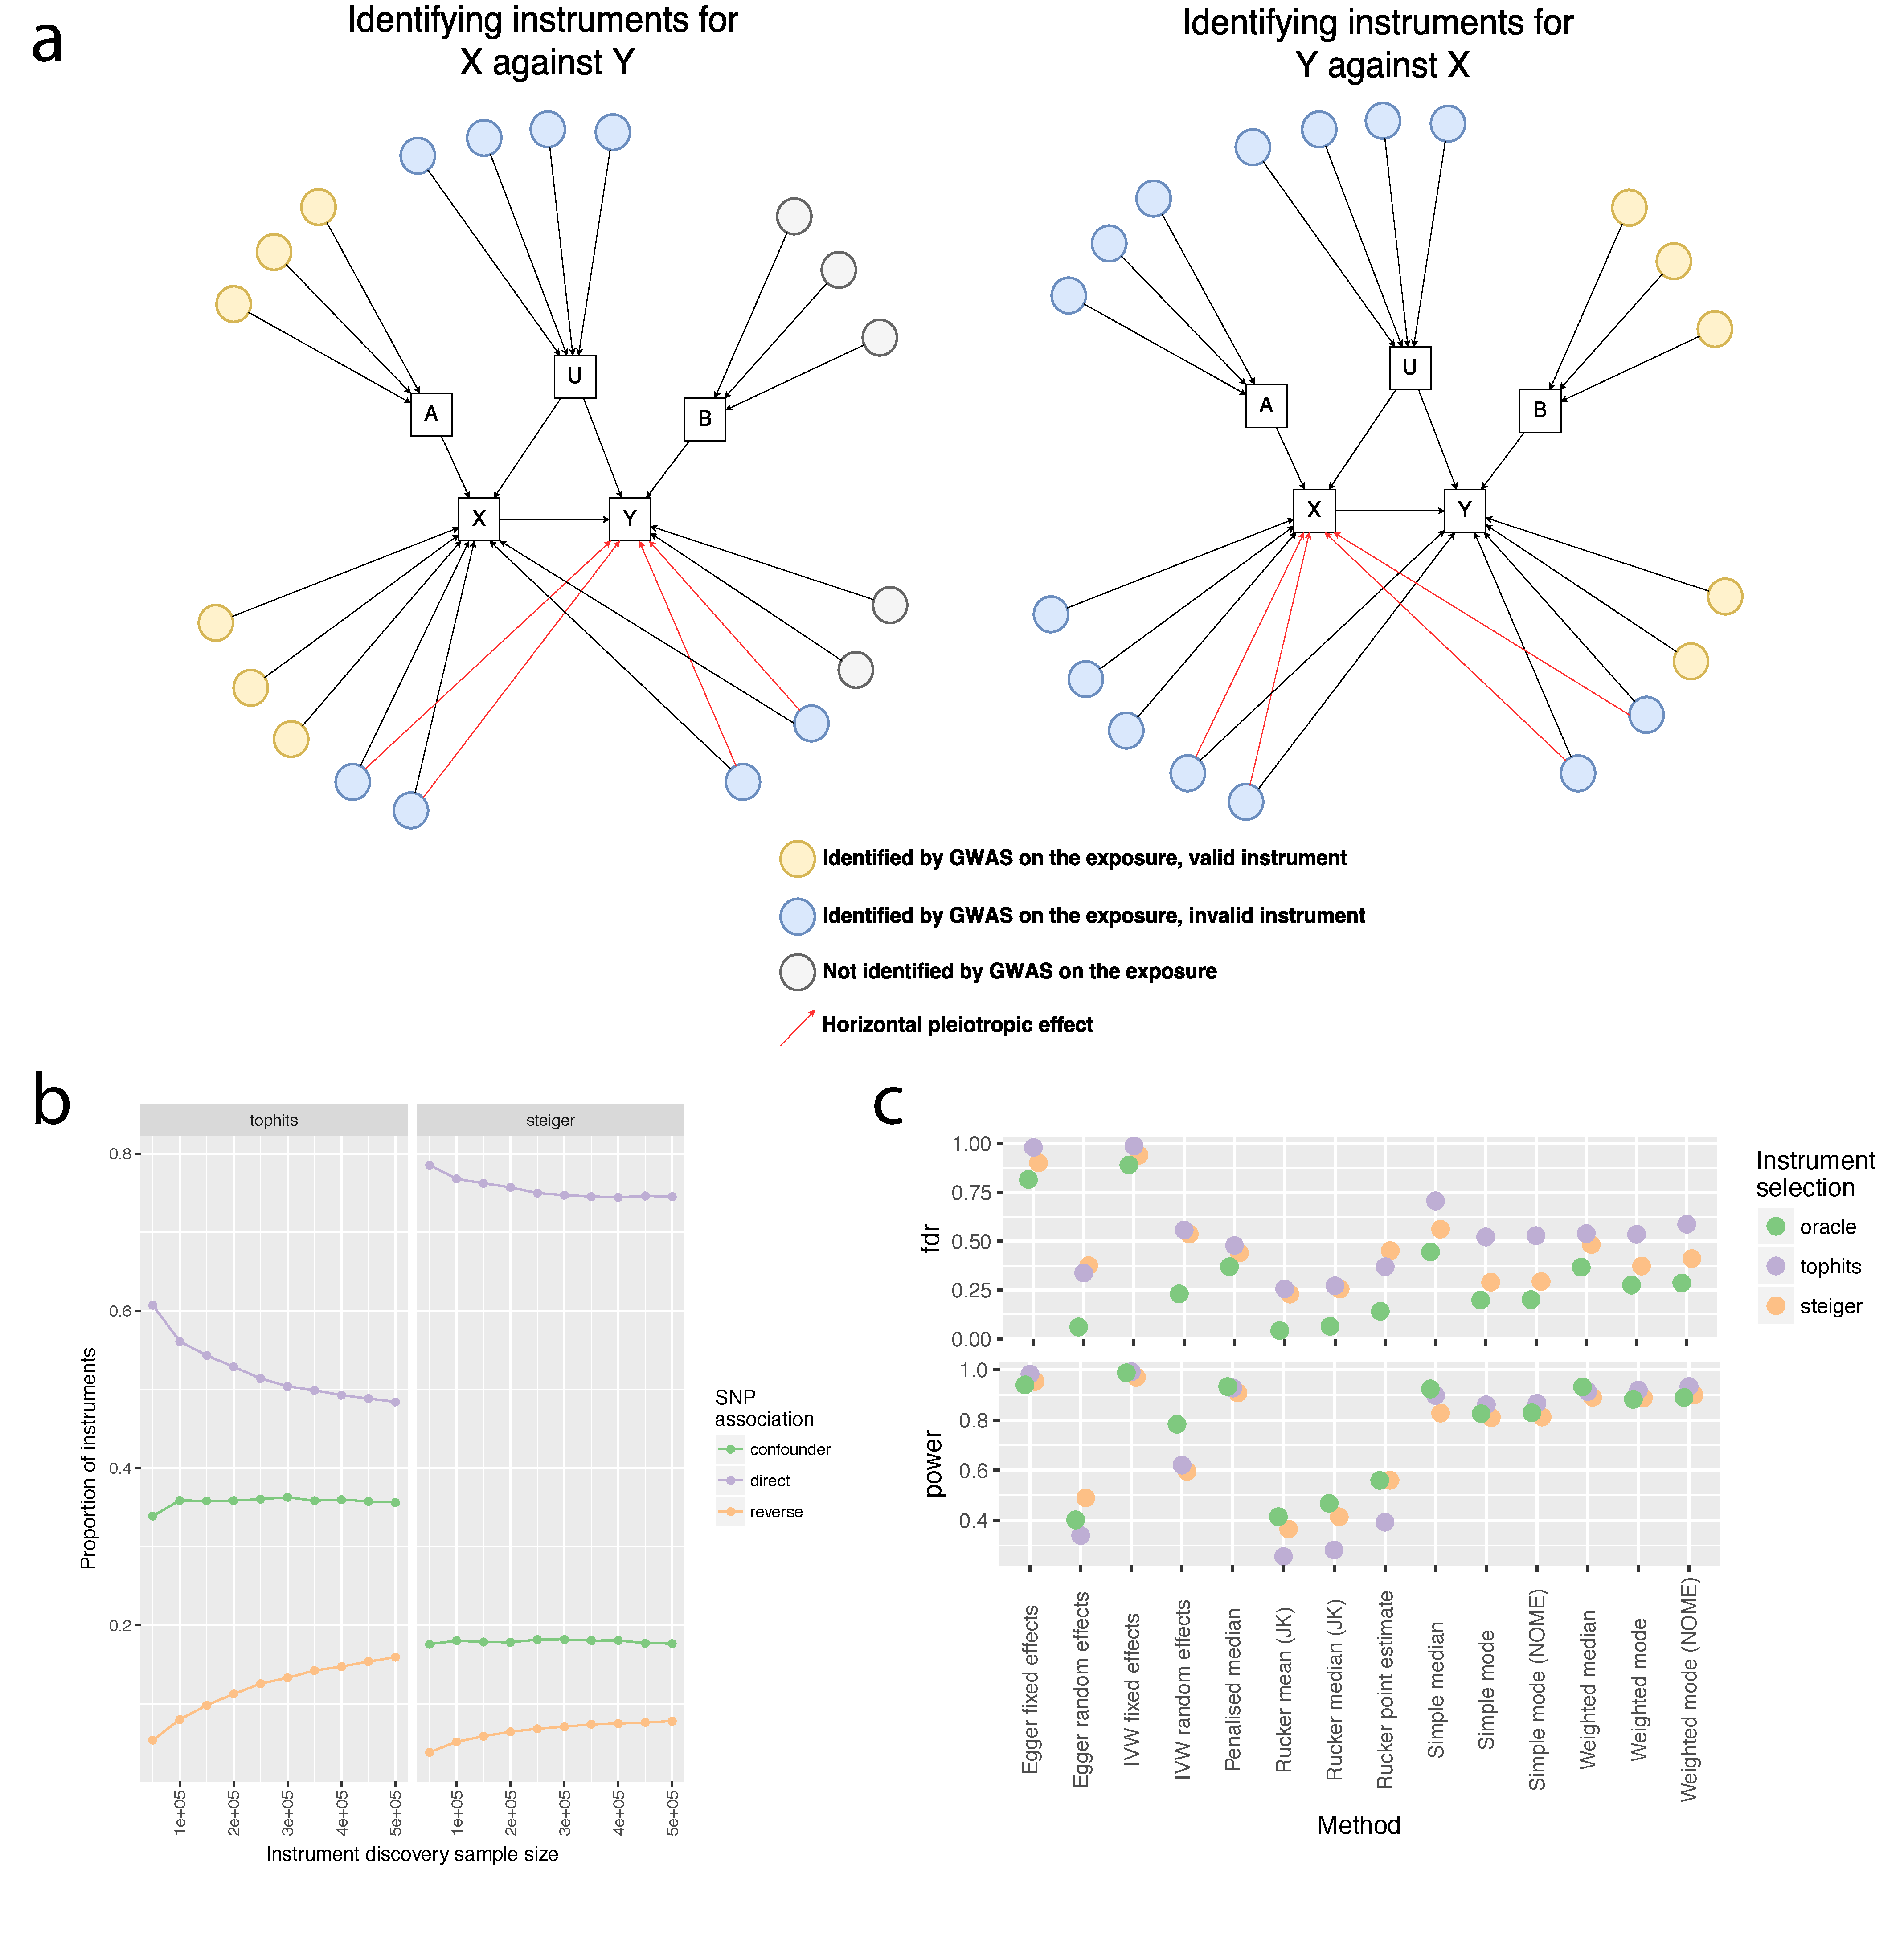
\includegraphics{images/fig1.pdf}

Figure 1: Simulations. a) Schematic of how GWAS with sufficient power
can lead to the selection of instrumental variables that are invalid. We
used arbitrary numbers of SNPs and confounders to simulate GWAS summary
datasets. b) Any SNP that has a direct influence on the exposure, or an
influence on a non-confounding intermediate variable, is considered a
`direct' effect. The y-axis shows the proportion of instruments selected
for analysis that are either direct associations with the exposure,
instruments for the outcome (reverse), or instruments for confounding
traits (confounder). The proportions are compared over a range of
different exposure discovery sample sizes (x-axis) and using either the
tophits approach (left) or the Steiger approach (right) for instrument
selection. c) Top: The false discovery rates from null simulations for
each of the 14 methods using either tophits, Steiger filtered variants,
or variants that are known to be directly associated with the exposure
(oracle, note that direct effects can still exhibit horizontal
pleiotropy in these simulations). Bottom: The statistical power to
detect true causal associations in the non-null simulations.

\newpage

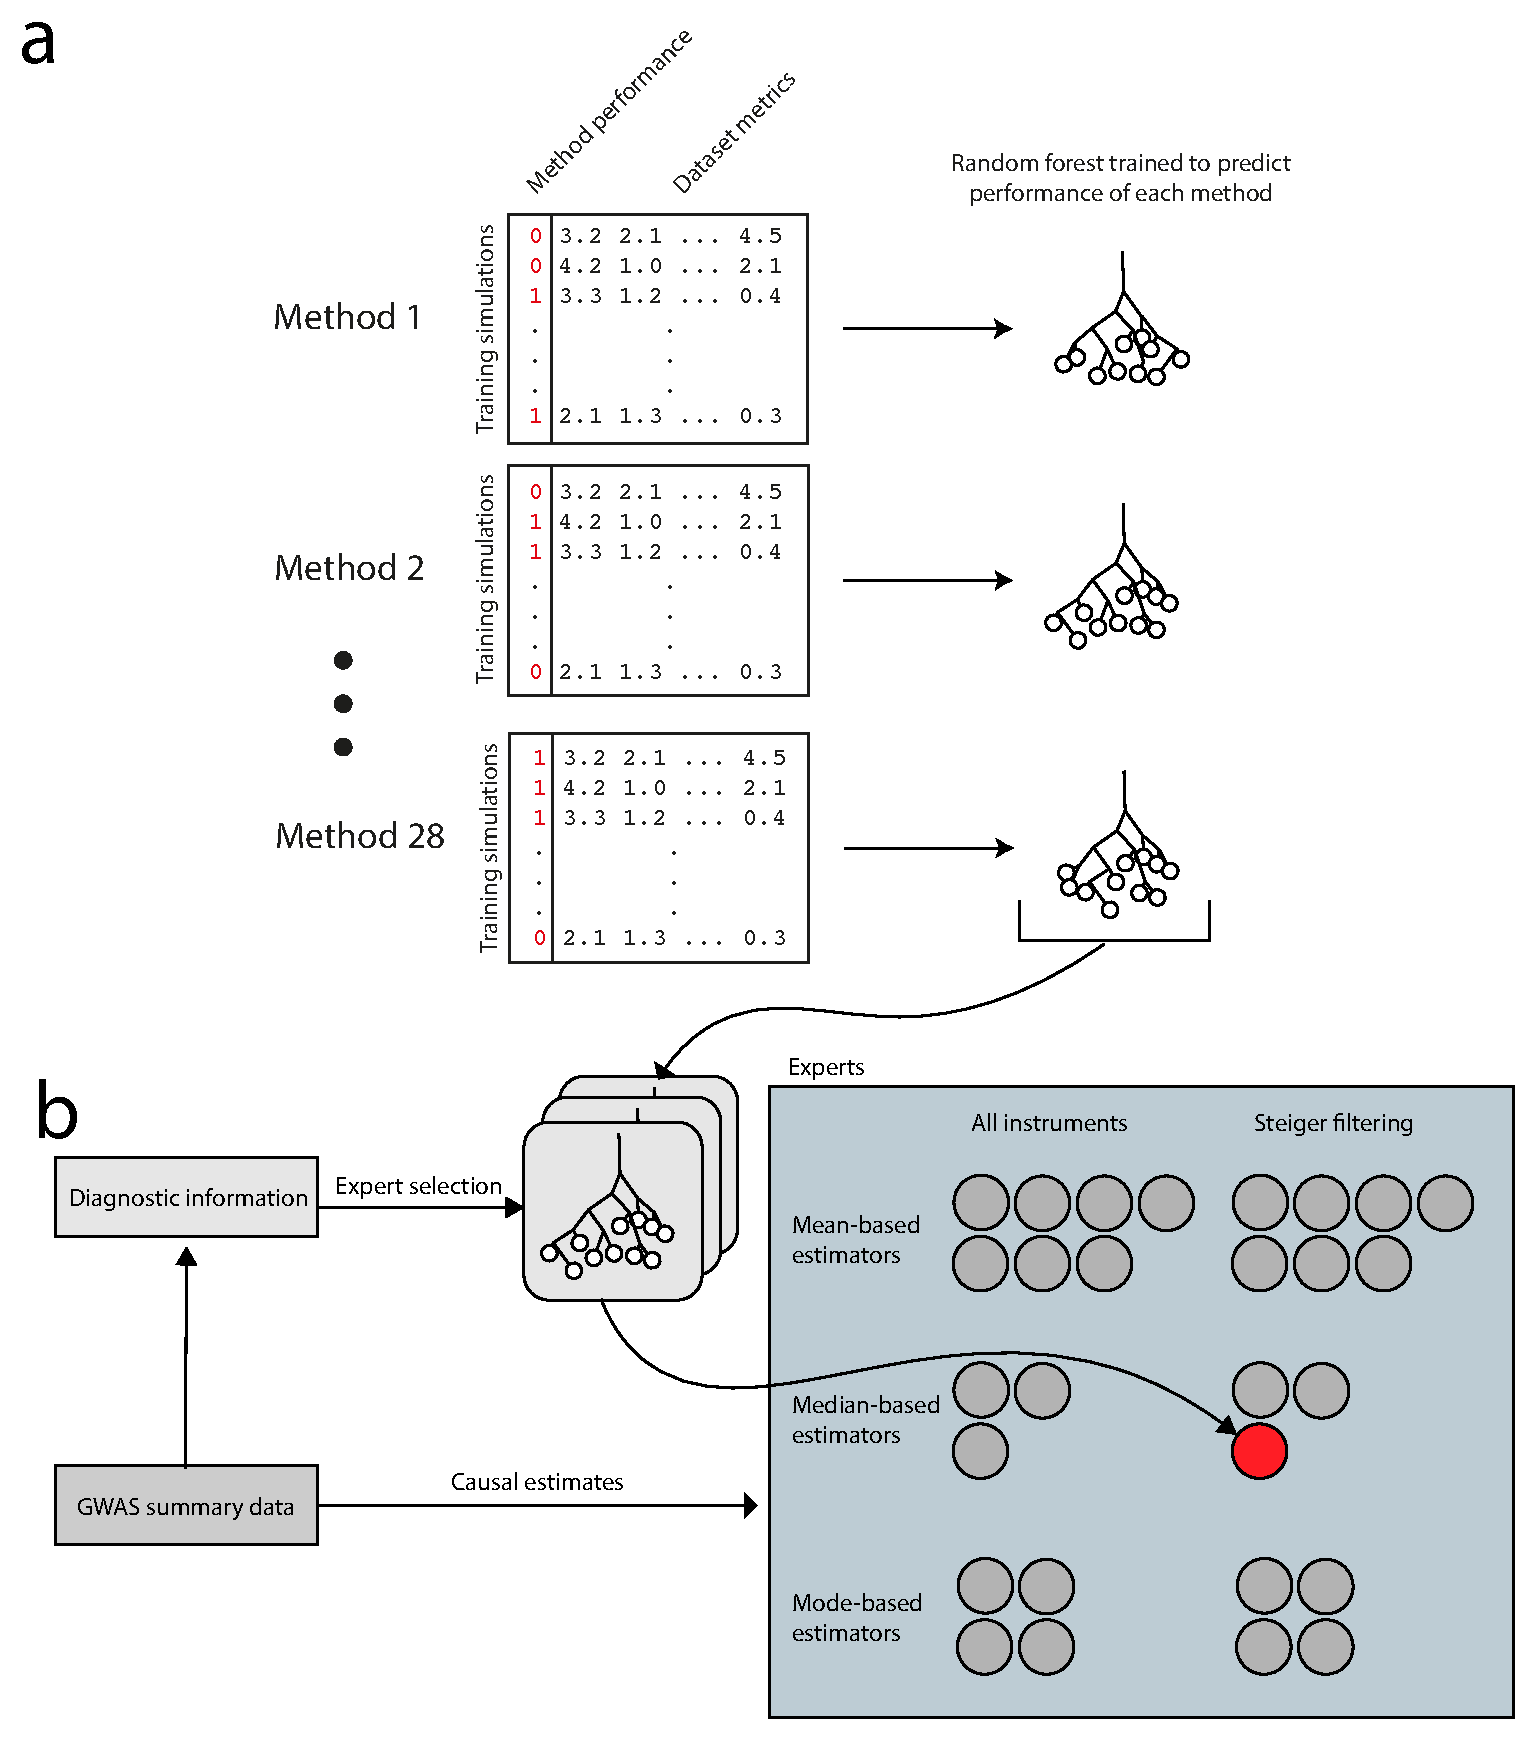
\includegraphics{images/fig2.pdf}

Figure 2: Mixture of experts. a) Training. Datasets are simulated that
have either null or non-null causal relationships, and causal estimates
are obtained from each of the 28 MR methods considered in this study. In
the toy datasets, the columns in black represent 53 metrics about each
of the 67,000 training simulations. The columns in red are specific to
each method, they represent how well that method performed in obtaining
the correct answer for each of the datasets. Random forests are used to
learn the parameter space of the 53 metrics in which a particular
dataset is likely to perform well. Together, this creates 28 random
forest decision trees, one for each method. b) Application. For a GWAS
summary dataset, our objective is to choose the method most likely to
return the correct causal estimate. Metrics are generated from the
dataset and fed into each of the 28 random forest decision trees. This
provides us with 28 performance predictions. Finally, we use the method
for which the performance prediction is highest.

\newpage

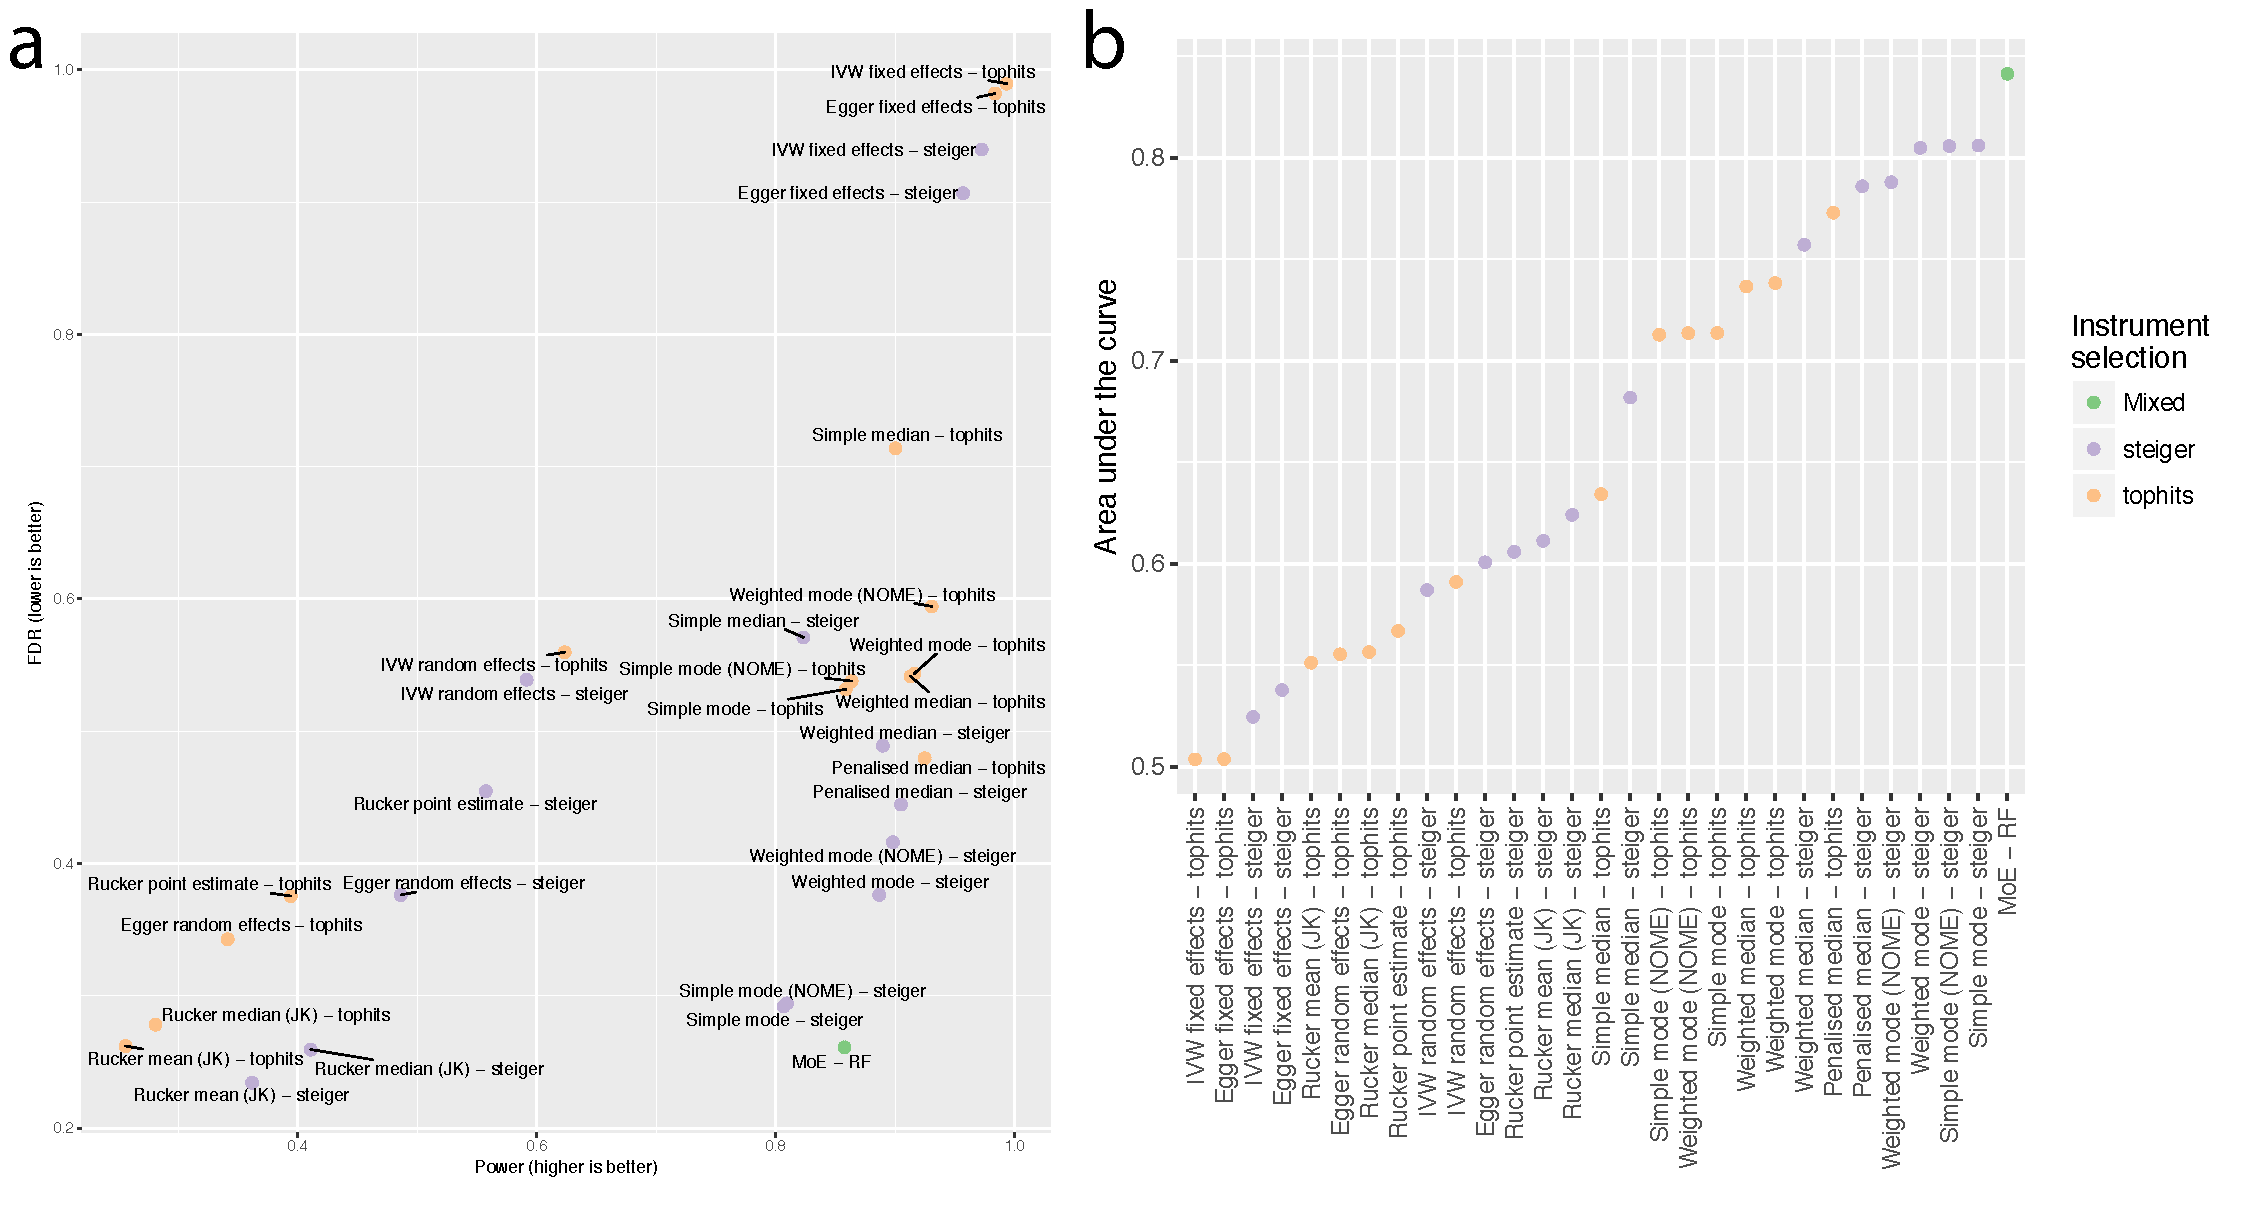
\includegraphics{images/fig3.pdf}

Figure 3: Performance of MoE against all other methods. a) The power for
non-null datasets is plotted against the FDR for null datasets for each
of the 28 methods, plus MoE. No single method achieved nominal FDR for
these simulations. b) Calculating the area under the ROC curve from the
values in (a) we plotted the performance in order from lowest to
highest. Under the assumption of pervasive horizontal pleiotropy, the
MoE approach is likely most effective than any other single method.

\newpage

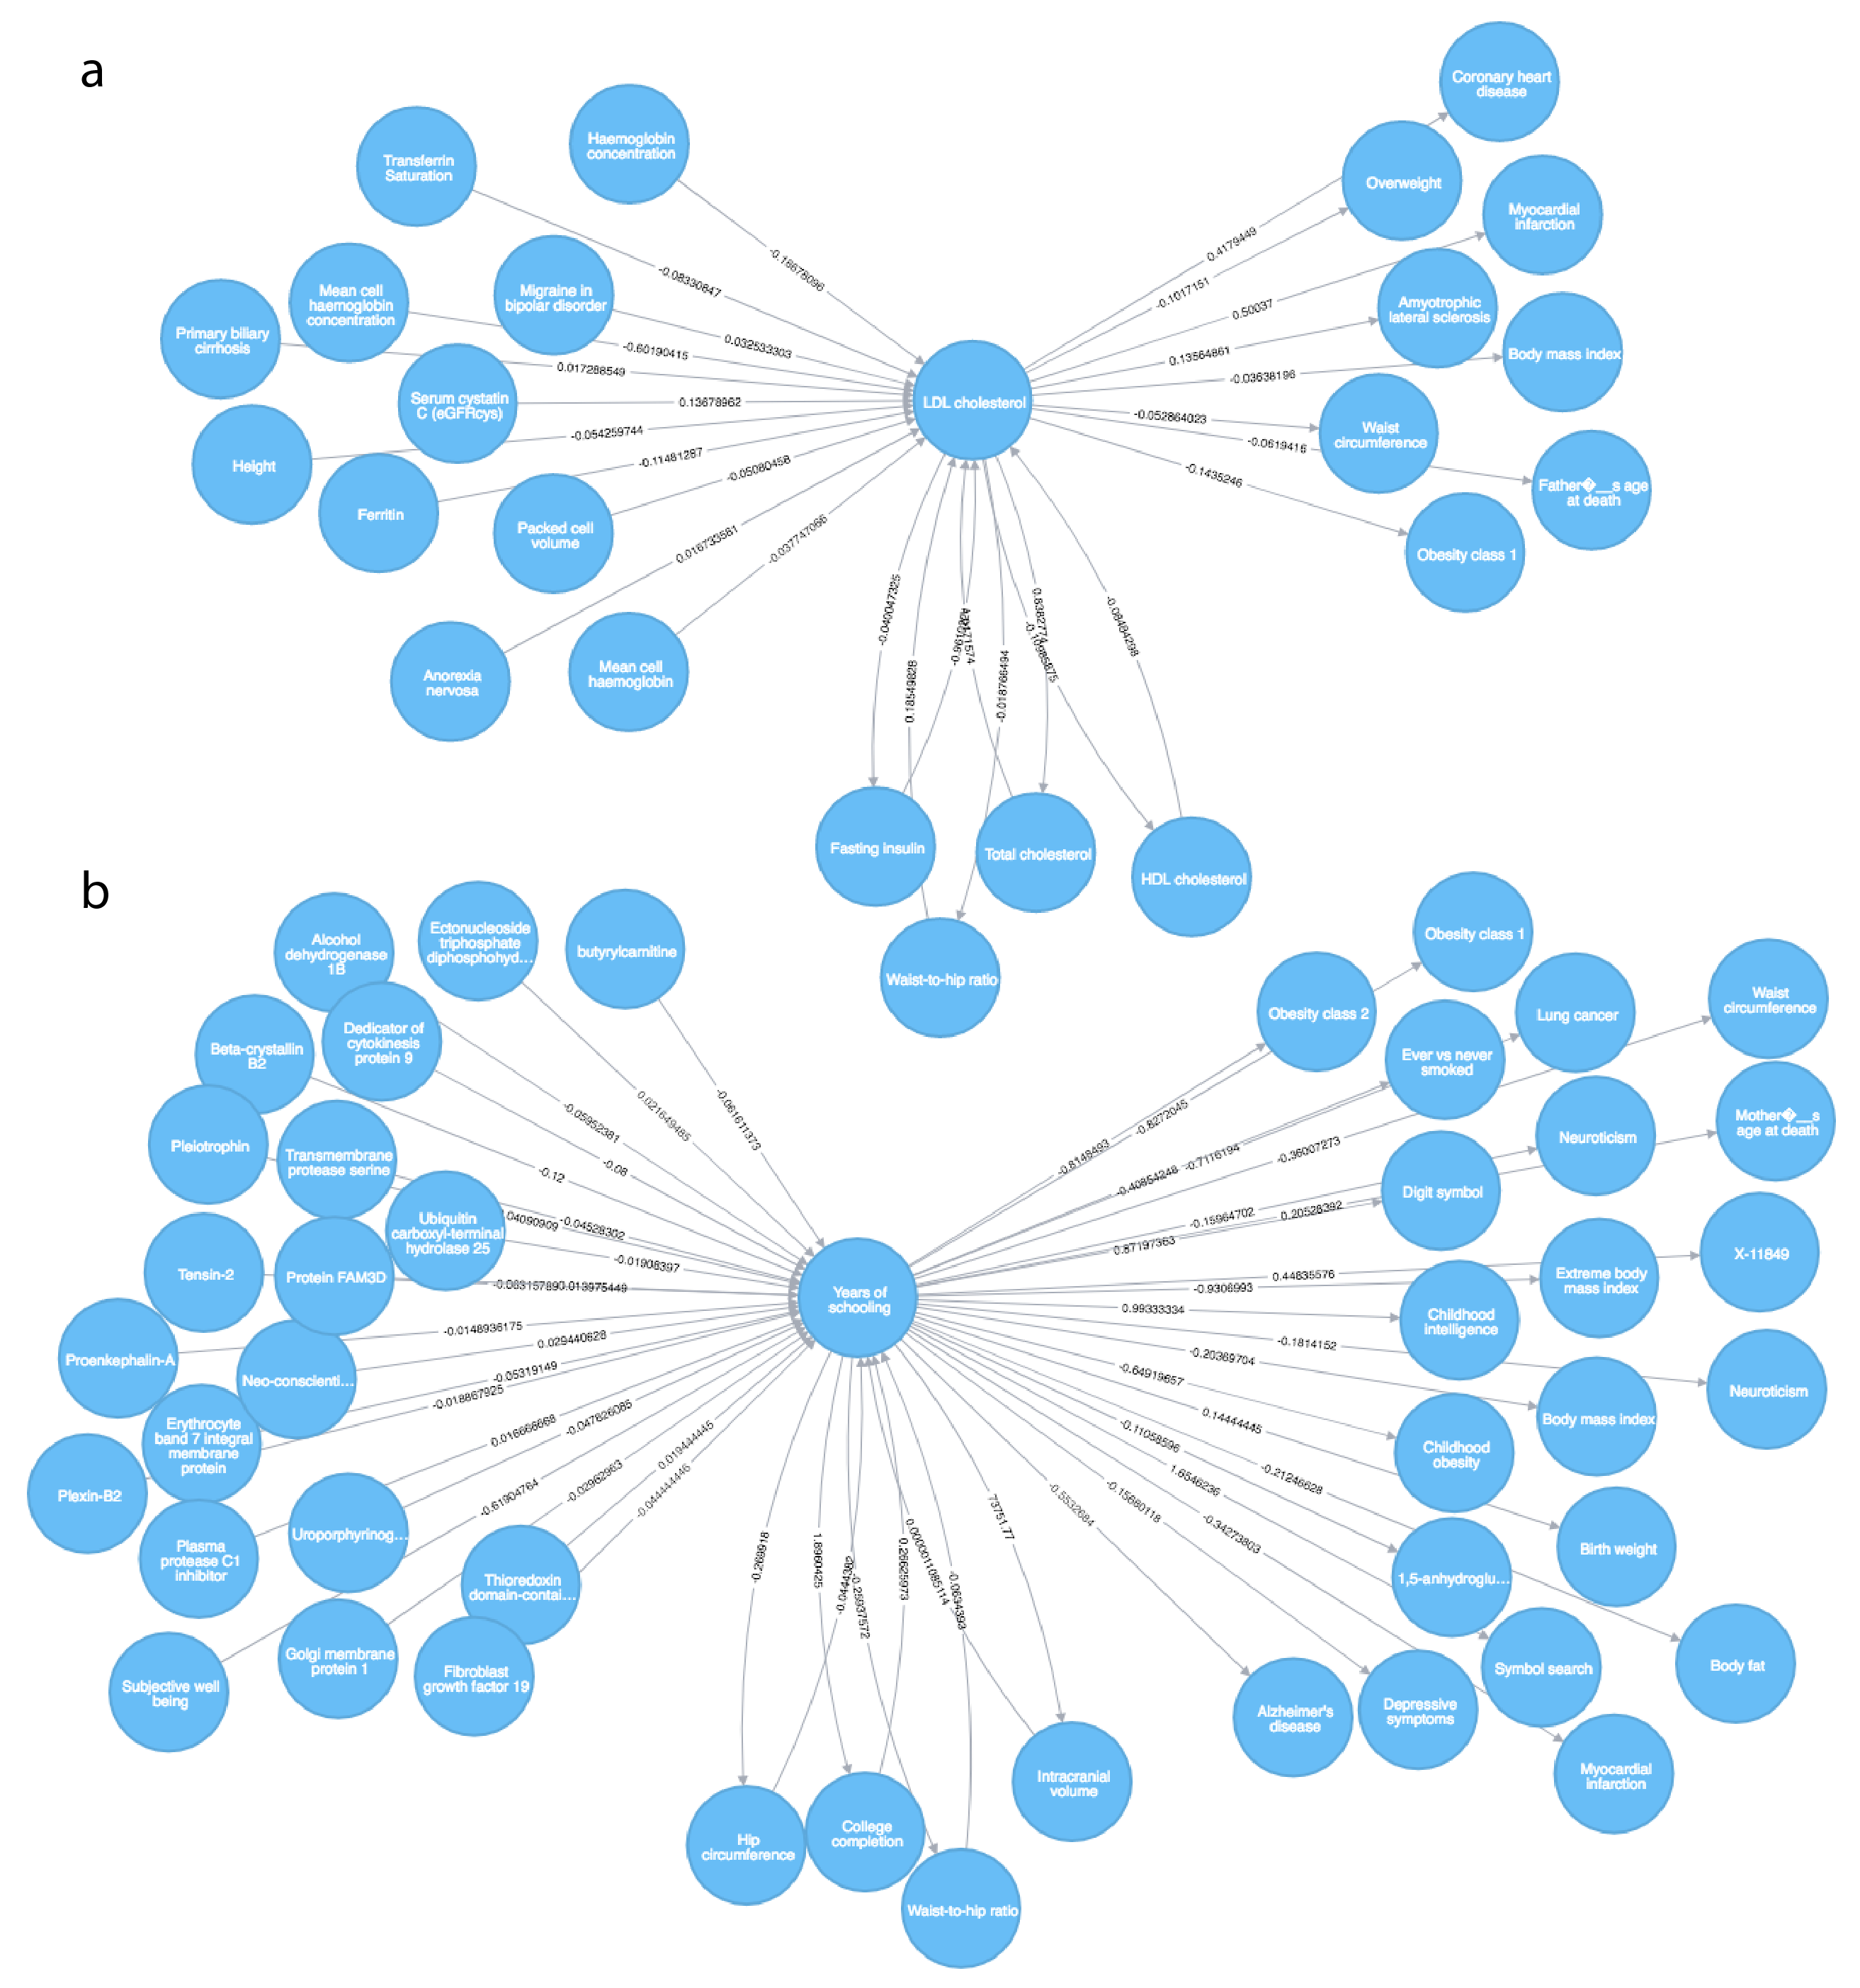
\includegraphics{images/fig4-01.png}

Figure 4: Lookup of causal associations involving a) LDL cholesterol and
b) Years of Schooling. In a) the nodes are filtered to not include those
obtained from the metabolomic studies (37,38). The arrows denote causal
direction and the values on the arrows denote the causal effect
estimate. Only those relationships are shown for which the
\(FDR < 0.05\).

\newpage

\subsection{Online methods}\label{online-methods}

\subsubsection{Steiger filtering}\label{steiger-filtering-1}

An approach to inferring the causal direction between phenotypes
recently developed (8) uses the following basic premise. If trait \(A\)
causes trait \(B\) then \(cor(g_{i}, A)^2 > cor(g_{i}, B)^2\) because
the \(cor(g_{i}, B)^2 = cor(A, B)^{2} cor(g_{i}, A)^{2}\). This will be
true under most circumstances, but some parameters of measurement error
or unmeasured confounding can lead to the inequality reversing
direction, as has been explored previously (8).

The Steiger test is applied to each variant in turn and we exclude any
\(g_{A}\) for which \(cor(g_{i}, A)^2 > cor(g_{i}, B)^2\), indicating
that it is unlikely to primarily associate with \(B\) relative to \(A\).
Similarly, for SNPs that influence confounders of \(A\) and \(B\) or
exhibit horizontal pleiotropy, the difference in \(cor(g_{i}, A)^2\) and
\(cor(g_{i}, B)^2\) will be reduced, increasing the likelihood of the
SNP being excluded because the Steiger Z-test is less likely to be
significant. Hence we also exclude any \(g_{A}\) for which the
\(cor(g, x)\) and \(cor(g, y)\) are not significantly different at an
arbitrary threshold of \(p > 0.05\).

To estimate \(cor(g, x)^2\), if \(x\) is continuous we obtain the
F-statistic from the reported p-value and sample size and then
\(cor(g, x)^2 = \frac{F}{N - 2 - F}\). If \(x\) is binary then we
estimate the variance of the underlying liability explained by the SNP,
\(cor(g, x)^2 = \frac{V_a}{V_a + V_e}\). Here, \(V_e = \pi^2/3\), and
\(V_a = 2\beta^2f(1-f)\), where \(\beta\) is the log odds ratio and
\(f\) is the allele frequency of the SNP in the population (52). \(f\)
can be estimated using the allele frequency of the SNP in an ascertained
sample by deriving the \(2 \times 2\) contingency table from the odds
ratio \(e^\beta\), allele frequency in the ascertained sample
\(f_{cc}\), and number of cases \(N_1\) and controls \(N_0\). A Z-score
to test the hypothesis that \(cor(g, x)\) and \(cor(g, y)\) are
significantly different can be generated using the Steiger test for
correlated correlations.

\subsubsection{Mixture of experts implementation for
MR}\label{mixture-of-experts-implementation-for-mr}

The mixture of experts approach seeks to use simulations to learn the
circumstances in which each of the 28 MR methods is likely to perform
most accurately. Having trained the model on simulations, new
summary-sets can be applied to obtain causal estimates from the method
that is predicted to be the most reliable for that summary-set.

\textbf{Training and testing simulations}

The MoE is trained using summary-sets generated from simulations (Figure
2a). Each \emph{summary-set} can be fed into any of the 28 experts to
obtain MR causal effects. The simulations used to generate these
summary-sets seek to cover a range of pleiotropic scenarios, including
where some proportion of SNPs exhibit directional or balanced horizontal
pleiotropy, or where SNPs influence confounding variables.

We simulate two individual level datasets for which there are \(N_x\)
and \(N_y\) samples, and \(M\) SNPs, where each SNP has effect allele
frequency of \(f_m \sim U(0.05, 0.95)\). These datasets are used to
obtain the SNP effects for the exposure trait \(x\) and the outcome
trait \(y\), respectively, to create summary-sets, using the following
sampling criteria:

\[
\begin{aligned}
N_x & = \{20000, ..., 500000\} \\
N_y & = \{20000, ..., 500000\} \\
K & = \{0, ..., 10\} \\
M_x & = \{1, ..., 200\} \\
M_y & = \{1, ..., 200\} \\
M_{u_k} & = \{5,..., 30\} \\
\end{aligned}
\]

The \(M = M_x + M_y + \sum{M_{u_k}}\) SNPs can influence \(x\) directly,
\(y\) directly, or some number of confounders \(u_{k}\) directly.
Phenotypes for \(x\) and \(y\) are constructed using

\[
x = \sum^{M_x}_{i}{\beta_{gx,x,i}g_{x,i}} + \sum^{M_y}_{j}{\beta_{gy,x,j}g_{y,j}} + \sum^{K}_{k}{\beta_{ux,k} u_{k}} + e_{x}
\]

where \(\beta_{gx,x}\) is the vector of effects of each of the \(M_x\)
SNPs that influence \(x\) primarily, \(\beta_{gy,x}\) is the vector of
effects for the \(M_y\) SNPs on \(x\), where the \(M_y\) SNPs influence
\(y\) primarily but exhibit horizontal pleiotropic effects on \(x\). We
allow some proportion of these effects to be 0. \(\beta_{ux}\) is the
vector of effects of each of the \(K\) confounders on \(x\). Each
\(u_{k}\) variable is constructed using

\[
u = \sum^{M_u}_{l}{\beta_{gu,l}g_{l}} + e_{l}
\]

and finally \(y\) is constructed using

\[
y = \beta_{x,y}x + \sum^{M_y}_{i}{\beta_{gy,y,j}g_{y,j}} + \sum^{M_x}_{j}{\beta_{gx,y,i}g_{x,i}} + \sum^{K}_{k}{\beta_{uy,k} u_{k}} + e_{y}
\]

where \(\beta_{x,y}\) is the causal effect of \(x\) on \(y\). We sample
the distribution of direct SNP effects using

\[
\begin{aligned}
\beta_{gx,x,i} & \sim N(0, \sigma^2_{gx,x}) \\
\sigma^2_{gx,x,i} & \sim U(0.01, 0.1) \\
\beta_{gy,y,j} ~ N(0, \sigma^2_{gy,y}) \\
\sigma^2_{gy,y,j} & \sim U(0.01, 0.1) \\
\end{aligned}
\]

Some proportion \(floor(MS_{x}/M)\) of \(g_x\) SNPs and
\(floor(MS_{y}/M)\) of \(g_y\) SNPs, where \(s_x\) and
\(s_y \sim U(0,1)\), exhibit horizontal pleiotropy with effects sampled
using

\[
\begin{aligned}
\beta_{gx,y,i*} & \sim N(\mu_{gx,y}, \sigma^2_{gx,y})  \\
\mu_{gx,y,i*} & \sim U(-0.005, 0.005) \\
\sigma^2_{gx,y,i*} & \sim U(0.001, 0.01) \\
\beta_{gy,x,j*} & \sim N(\mu_{gy,x}, \sigma^2_{gy,x}) \\
\mu_{gy,x,j*} & \sim U(-0.005, 0.005) \\
\sigma^2_{gy,x,j*} & \sim U(0.001, 0.01) \\
\end{aligned}
\]

The genetic influences on each of the confounders are sampled using

\[
\begin{aligned}
\beta_{gu,u,l} & \sim N(0, \sigma^2_{gu,u}) \\
\sigma^2_{gu,u,l} & \sim U(0.01, 0.1) \\
\end{aligned}
\]

The influence of each confounder on \(x\) and \(y\) is obtained using

\[
\begin{aligned}
\beta_{u,x} & \sim N(0, \sigma^{2}_{u,x}) \\
\beta_{u,y} & \sim N(0, \sigma^{2}_{u,y}) \\
\end{aligned}
\]

Finally, 20\% of the simulations have a null effect of
\(\beta_{x,y} = 0\), while the other remaining 80\% have a true effect
sampled from

\[
\begin{aligned}.
\beta_{x,y} & \sim N(0, \sigma^2_{x,y}) \\
\sigma^2_{x,y} & \sim U(0.001, 0.1) \\
\end{aligned}
\]

For each simulation we used linear regression to estimate the genetic
effect of each SNP \(M\) on \(x\) in sample 1, and each SNP \(M\) on
\(y\) in sample 2. We then perform MR analysis in both directions,
mimicking GWAS by retaining SNPs that have \(p < 5e-8\) in sample 1 to
perform MR of \(x\) on \(y\) (the true causal direction for non-null
simulations), and retaining SNPs that have \(p < 5e-8\) in sample 2 to
perform MR of \(y\) on \(x\) (the reverse causal direction for non-null
simulations). We treat the summary data (effect sizes and standard
errors) used for estimating \(x \rightarrow y\) the summary data used
for estimating \(y \rightarrow x\) as two separate summary-sets. Hence,
for each simulation two summary-sets are generated which are analysed to
produce 28 MR estimates each. We performed 100,000 simulations using
these parameters, resulting in 200,000 summary-sets.

\textbf{Optimisation function}

We aim to maximise statistical power for summary-sets where
\(\beta_{x,y} \neq 0\) and minimise false discovery rates for
summary-sets where \(\beta_{x,y} = 0\). To train random forest decision
trees to predict performance for a particular method
\(h(O_{w,d}, \textbf{z}_{d})\) is generated where the training set of
input metrics for summary-set \(d\) is \(\textbf{z}_{d}\) and the
response (optimisation function) is

\[
    O_{w,d} = 
\begin{cases}
    1,   & \text{if } \beta_{x,y} \neq 0 \text{ and } p_{m,d} < 0.01\\
    1,   & \text{if } \beta_{x,y} = 0 \text{ and } p_{m,d} > 0.1 \\
    0,   & \text{otherwise}
\end{cases}
\]

where \(p_{m,d}\) is the p-value for method \(m\) on summary-set \(d\).

\textbf{Strategy}

For each training summary-set we record a set of 53 metrics
\(\textbf{z}_{d}\) (Supplementary table 3), and an outcome \(O_{w,d}\),
which is a measure of how well that method performed for each particular
simulated summary-set. For each of our 28 methods, we need to create a
model that predicts the performance of the method based on metrics
generated from a summary-set. To do this, for each method we train a
random decision forest to predict that method's performance using the
summary-set's metrics. The random forest approach is well suited to this
problem because there are likely to be non-continuous combinations of
different metrics that improve on prediction over, for example, a simple
linear model that does not learn about interactions.

As a simple hypothetical example - if a summary-set exhibits a single
outlier but is otherwise exhibiting no heterogeneity then the following
methods could arguably perform well:

\begin{itemize}
\tightlist
\item
  an IVW fixed effects analysis with the outlier removed, should the
  Steiger test be able to detect the outlier
\item
  a median based approach
\item
  a mode based approach
\end{itemize}

deciding between these methods requires finding, in general, which will
minimise false discovery rates and maximise true positive rates for that
particular scenario. In this example the IVW with Steiger filtering
would likely be the clear winner because of its superior statistical
power. Countless other scenarios could arise. For example if 100\% of
instruments are invalid but the InSIDE assumptio is met then the
MR-Egger is likely to be most effective; if 40\% of instruments are
invalid then a median-based approach is likely most effective; and if
80\% of instruments are invalid then a mode-based approach is likely
most effective.

Having generated random forest decision trees for each of the 28 methods
using 133,000 of the simulations, we then applied them to the remaining
67,000 summary-sets to predict which method would have the highest
performance for each of the remaining summary-sets. Finally we compare
the performance of the method selected by the MoE against all remaining
methods. The default settings for the \texttt{randomForest} package in R
(53) were used to train the models. MR-MoE 1.0 is implemented in the
TwoSampleMR R package available at
\href{https://github.com/MRCIEU/TwoSampleMR}{github.com/MRCIEU/TwoSampleMR}
(12).

\subsection{References}\label{references}

\raggedright

\hypertarget{refs}{}
\hypertarget{ref-DaveySmith2003}{}
1. Davey Smith G, Ebrahim S. 'Mendelian randomization': can genetic
epidemiology contribute to understanding environmental determinants of
disease? International Journal of Epidemiology {[}Internet{]}. 2003
Feb;32(1):1--22. Available from:
\url{http://www.ije.oxfordjournals.org/cgi/doi/10.1093/ije/dyg070}

\hypertarget{ref-DaveySmithHemani2014}{}
2. Davey Smith G, Hemani G. Mendelian randomization: genetic anchors for
causal inference in epidemiological studies. Human molecular genetics.
2014 Jul;23(R1):R89-----R98.

\hypertarget{ref-Holmes2017}{}
3. Holmes MV, Ala-Korpela M, Smith GD. Mendelian randomization in
cardiometabolic disease: challenges in evaluating causality. Nature
Reviews Cardiology {[}Internet{]}. 2017 Jun; Available from:
\href{http://www.ncbi.nlm.nih.gov/pubmed/28569269\%20http://www.nature.com/doifinder/10.1038/nrcardio.2017.78}{http://www.ncbi.nlm.nih.gov/pubmed/28569269 http://www.nature.com/doifinder/10.1038/nrcardio.2017.78}

\hypertarget{ref-Bowden2015}{}
4. Bowden J, Davey Smith G, Burgess S. Mendelian randomization with
invalid instruments: effect estimation and bias detection through Egger
regression. International Journal of Epidemiology. 2015;44(2):512--25.

\hypertarget{ref-Bowden2016b}{}
5. Bowden J, Davey Smith G, Haycock PC, Burgess S. Consistent Estimation
in Mendelian Randomization with Some Invalid Instruments Using a
Weighted Median Estimator. Genetic Epidemiology {[}Internet{]}. 2016
May;40(4):304--14. Available from:
\href{http://www.ncbi.nlm.nih.gov/pubmed/27061298\%20http://www.pubmedcentral.nih.gov/articlerender.fcgi?artid=PMC4849733\%20http://doi.wiley.com/10.1002/gepi.21965}{http://www.ncbi.nlm.nih.gov/pubmed/27061298 http://www.pubmedcentral.nih.gov/articlerender.fcgi?artid=PMC4849733 http://doi.wiley.com/10.1002/gepi.21965}

\hypertarget{ref-Bowden2017}{}
6. Bowden J, Del~Greco~M F, Minelli C, Davey Smith G, Sheehan N,
Thompson J. A framework for the investigation of pleiotropy in
two-sample summary data Mendelian randomization. Statistics in Medicine
{[}Internet{]}. 2017; Available from:
\url{http://doi.wiley.com/10.1002/sim.7221}

\hypertarget{ref-Hartwig2017}{}
7. Hartwig FP, Davey Smith G, Bowden J. Robust Inference In Two-Sample
Mendelian Randomisation Via The Zero Modal Pleiotropy Assumption.
bioRxiv {[}Internet{]}. 2017; Available from:
\url{http://biorxiv.org/content/early/2017/04/10/126102}

\hypertarget{ref-Hemani2017}{}
8. Hemani G, Tilling K, Davey Smith G. Orienting The Causal Relationship
Between Imprecisely Measured Traits Using Genetic Instruments. bioRxiv
{[}Internet{]}. 2017; Available from:
\url{http://biorxiv.org/content/early/2017/03/15/117101}

\hypertarget{ref-Verbanck2017}{}
9. Verbanck M, Chen C-Y, Neale B, Do R. Widespread pleiotropy confounds
causal relationships between complex traits and diseases inferred from
Mendelian randomization. bioRxiv {[}Internet{]}. 2017; Available from:
\url{http://www.biorxiv.org/content/early/2017/06/30/157552}

\hypertarget{ref-Hindorff2010}{}
10. Hindorff LA, Junkins HA, Hall PN, Mehta JP, Manolio TA. A Catalog of
Published Genome-Wide Association Studies, available at
http://www.genome.gov/gwastudies. Accessed 12/10/2010. 2010.

\hypertarget{ref-Pierce2013}{}
11. Pierce BL, Burgess S. Efficient design for Mendelian randomization
studies: subsample and 2-sample instrumental variable estimators.
American journal of epidemiology {[}Internet{]}. 2013
Oct;178(7):1177--84. Available from:
\href{http://www.pubmedcentral.nih.gov/articlerender.fcgi?artid=3783091\%7B/\&\%7Dtool=pmcentrez\%7B/\&\%7Drendertype=abstract}{http://www.pubmedcentral.nih.gov/articlerender.fcgi?artid=3783091\{\textbackslash{}\&\}tool=pmcentrez\{\textbackslash{}\&\}rendertype=abstract}

\hypertarget{ref-Hemani2016}{}
12. Hemani G, Zheng J, Wade KH, Laurin C, Elsworth B, Burgess S, et al.
MR-Base: a platform for systematic causal inference across the phenome
using billions of genetic associations. BioRxiv. 2016;10.1101/07.

\hypertarget{ref-Zhu2017}{}
13. Zhu Z, Zheng Z, Zhang F, Wu Y, Trzaskowski M, Maier R, et al. Causal
associations between risk factors and common diseases inferred from GWAS
summary data. bioRxiv {[}Internet{]}. 2017; Available from:
\url{http://www.biorxiv.org/content/early/2017/07/26/168674}

\hypertarget{ref-Wright1968}{}
14. Wright S. Evolution and the Genetics of Populations. In: Evolution
and the genetics of populations. Chicago: University of Chicago Press;
1968.

\hypertarget{ref-Wagner2011}{}
15. Wagner GP, Zhang J. The pleiotropic structure of the
genotype--phenotype map: the evolvability of complex organisms. Nature
Reviews Genetics {[}Internet{]}. 2011 Mar;12(3):204--13. Available from:
\url{http://www.nature.com/doifinder/10.1038/nrg2949}

\hypertarget{ref-Hill2012a}{}
16. Hill WG, Zhang X-S. Assessing pleiotropy and its evolutionary
consequences: pleiotropy is not necessarily limited, nor need it hinder
the evolution of complexity. Nature Reviews Genetics {[}Internet{]}.
2012 Feb;13(4):296. Available from:
\url{http://www.ncbi.nlm.nih.gov/pubmed/22349131}

\hypertarget{ref-Hartwig2016}{}
17. Hartwig FP, Davies NM, Hemani G, Davey Smith G. Two-sample Mendelian
randomization: avoiding the downsides of a powerful, widely applicable
but potentially fallible technique. International Journal of
Epidemiology {[}Internet{]}. 2016 Dec;45(6):1717--26. Available from:
\url{https://academic.oup.com/ije/article-lookup/doi/10.1093/ije/dyx028}

\hypertarget{ref-Xu2017}{}
18. Xu L, Lin SL, Schooling CM. A Mendelian randomization study of the
effect of calcium on coronary artery disease, myocardial infarction and
their risk factors. Scientific Reports {[}Internet{]}. 2017 Feb;7:42691.
Available from:
\href{http://www.ncbi.nlm.nih.gov/pubmed/28195141\%20http://www.pubmedcentral.nih.gov/articlerender.fcgi?artid=PMC5307362\%20http://www.nature.com/articles/srep42691}{http://www.ncbi.nlm.nih.gov/pubmed/28195141 http://www.pubmedcentral.nih.gov/articlerender.fcgi?artid=PMC5307362 http://www.nature.com/articles/srep42691}

\hypertarget{ref-Larsson2017}{}
19. Larsson SC, Burgess S, Michaëlsson K, TB H, WH C, Y P. Association
of Genetic Variants Related to Serum Calcium Levels With Coronary Artery
Disease and Myocardial Infarction. JAMA {[}Internet{]}. 2017
Jul;318(4):371. Available from:
\url{http://jama.jamanetwork.com/article.aspx?doi=10.1001/jama.2017.8981}

\hypertarget{ref-Prins2016}{}
20. Prins BP, Abbasi A, Wong A, Vaez A, Nolte I, Franceschini N, et al.
Investigating the Causal Relationship of C-Reactive Protein with 32
Complex Somatic and Psychiatric Outcomes: A Large-Scale Cross-Consortium
Mendelian Randomization Study. Hay PJ, editor. PLOS Medicine
{[}Internet{]}. 2016 Jun;13(6):e1001976. Available from:
\href{http://www.ncbi.nlm.nih.gov/pubmed/27327646\%20http://www.pubmedcentral.nih.gov/articlerender.fcgi?artid=PMC4915710\%20http://dx.plos.org/10.1371/journal.pmed.1001976}{http://www.ncbi.nlm.nih.gov/pubmed/27327646 http://www.pubmedcentral.nih.gov/articlerender.fcgi?artid=PMC4915710 http://dx.plos.org/10.1371/journal.pmed.1001976}

\hypertarget{ref-Inoshita2016}{}
21. Inoshita M, Numata S, Tajima A, Kinoshita M, Umehara H, Nakataki M,
et al. A significant causal association between C-reactive protein
levels and schizophrenia. Scientific Reports {[}Internet{]}. 2016
Sep;6(1):26105. Available from:
\href{http://www.ncbi.nlm.nih.gov/pubmed/27193331\%20http://www.pubmedcentral.nih.gov/articlerender.fcgi?artid=PMC4872134\%20http://www.nature.com/articles/srep26105}{http://www.ncbi.nlm.nih.gov/pubmed/27193331 http://www.pubmedcentral.nih.gov/articlerender.fcgi?artid=PMC4872134 http://www.nature.com/articles/srep26105}

\hypertarget{ref-Solovieff2013}{}
22. Solovieff N, Cotsapas C, Lee PH, Purcell SM, Smoller JW. Pleiotropy
in complex traits: challenges and strategies. Nat Rev Genet
{[}Internet{]}. 2013 Jun;14(7):483--95. Available from:
\href{http://www.nature.com/doifinder/10.1038/nrg3461\%20http://dx.doi.org/10.1038/nrg3461\%2010.1038/nrg3461}{http://www.nature.com/doifinder/10.1038/nrg3461 http://dx.doi.org/10.1038/nrg3461 10.1038/nrg3461}

\hypertarget{ref-Hodgkin1998}{}
23. Hodgkin J. Seven types of pleiotropy. The International journal of
developmental biology {[}Internet{]}. 1998;42(3):501--5. Available from:
\url{http://www.ncbi.nlm.nih.gov/pubmed/9654038}

\hypertarget{ref-Paaby2013}{}
24. Paaby AB, Rockman MV. The many faces of pleiotropy {[}Internet{]}.
Vol. 29. 2013. pp. 66--73. Available from:
\href{http://www.ncbi.nlm.nih.gov/pubmed/23140989\%20http://www.pubmedcentral.nih.gov/articlerender.fcgi?artid=PMC3558540\%20http://linkinghub.elsevier.com/retrieve/pii/S0168952512001692}{http://www.ncbi.nlm.nih.gov/pubmed/23140989 http://www.pubmedcentral.nih.gov/articlerender.fcgi?artid=PMC3558540 http://linkinghub.elsevier.com/retrieve/pii/S0168952512001692}

\hypertarget{ref-Hu2016}{}
25. Hu JX, Thomas CE, Brunak S. Network biology concepts in complex
disease comorbidities. Nature reviews Genetics {[}Internet{]}.
2016;17(10):615--29. Available from:
\href{http://www.nature.com/doifinder/10.1038/nrg.2016.87\%7B/\%\%7D5Cnhttp://www.ncbi.nlm.nih.gov/pubmed/27498692}{http://www.nature.com/doifinder/10.1038/nrg.2016.87\{\textbackslash{}\%\}5Cnhttp://www.ncbi.nlm.nih.gov/pubmed/27498692}

\hypertarget{ref-Burgess2015b}{}
26. Burgess S, Scott RA, Timpson NJ, Davey Smith G, Thompson SG, EPIC-
InterAct Consortium. Using published data in Mendelian randomization: a
blueprint for efficient identification of causal risk factors. European
Journal of Epidemiology {[}Internet{]}. 2015 Jul;30(7):543--52.
Available from:
\href{http://www.ncbi.nlm.nih.gov/pubmed/25773750\%20http://www.pubmedcentral.nih.gov/articlerender.fcgi?artid=PMC4516908\%20http://link.springer.com/10.1007/s10654-015-0011-z}{http://www.ncbi.nlm.nih.gov/pubmed/25773750 http://www.pubmedcentral.nih.gov/articlerender.fcgi?artid=PMC4516908 http://link.springer.com/10.1007/s10654-015-0011-z}

\hypertarget{ref-Rucker2011}{}
27. Rucker G, Schwarzer G, Carpenter JR, Binder H, Schumacher M.
Treatment-effect estimates adjusted for small-study effects via a limit
meta-analysis. Biostatistics {[}Internet{]}. 2011 Jan;12(1):122--42.
Available from:
\href{http://www.ncbi.nlm.nih.gov/pubmed/20656692\%20https://academic.oup.com/biostatistics/article-lookup/doi/10.1093/biostatistics/kxq046}{http://www.ncbi.nlm.nih.gov/pubmed/20656692 https://academic.oup.com/biostatistics/article-lookup/doi/10.1093/biostatistics/kxq046}

\hypertarget{ref-Han2008}{}
28. Han C. Detecting invalid instruments using L 1-GMM. Economics
Letters. 2008;101(3):285--7.

\hypertarget{ref-Kang2016}{}
29. Kang H, Zhang A, Cai TT, Small DS. Instrumental Variables Estimation
With Some Invalid Instruments and its Application to Mendelian
Randomization. Journal of the American Statistical Association.
2016;111(513):132--44.

\hypertarget{ref-Steiger1980}{}
30. Steiger JH. Tests for comparing elements of a correlation matrix.
Psychological Bulletin. 1980;87(2):245--51.

\hypertarget{ref-Corbin2016}{}
31. Corbin LJ, Richmond RC, Wade KH, Burgess S, Bowden J, Smith GD, et
al. BMI as a Modifiable Risk Factor for Type 2 Diabetes: Refining and
Understanding Causal Estimates Using Mendelian Randomization. Diabetes
{[}Internet{]}. 2016 Oct;65(10):3002--7. Available from:
\href{http://www.ncbi.nlm.nih.gov/pubmed/27402723\%20http://www.pubmedcentral.nih.gov/articlerender.fcgi?artid=PMC5279886}{http://www.ncbi.nlm.nih.gov/pubmed/27402723 http://www.pubmedcentral.nih.gov/articlerender.fcgi?artid=PMC5279886}

\hypertarget{ref-white2016plasma}{}
32. White J, Sofat R, Hemani G, Shah T, Engmann J, Dale C, et al. Plasma
urate concentration and risk of coronary heart disease: a Mendelian
randomisation analysis. The Lancet Diabetes \& Endocrinology. 2016;

\hypertarget{ref-Jordan1994}{}
33. Jordan MI, Jacobs RA. Hierarchical Mixtures of Experts and the EM
Algorithm. Neural Computation {[}Internet{]}. 1994 Mar;6(2):181--214.
Available from:
\url{http://www.mitpressjournals.org/doi/10.1162/neco.1994.6.2.181}

\hypertarget{ref-brazdil2008metalearning}{}
34. Brazdil P, Carrier CG, Soares C, Vilalta R. Metalearning:
Applications to data mining. Springer Science \& Business Media; 2008.

\hypertarget{ref-smith2009cross}{}
35. Smith-Miles KA. Cross-disciplinary perspectives on meta-learning for
algorithm selection. ACM Computing Surveys (CSUR). 2009;41(1):6.

\hypertarget{ref-lemke2015metalearning}{}
36. Lemke C, Budka M, Gabrys B. Metalearning: a survey of trends and
technologies. Artificial intelligence review. 2015;44(1):117--30.

\hypertarget{ref-Shin2014}{}
37. Shin S-Y, Fauman EB, Petersen A-K, Krumsiek J, Santos R, Huang J, et
al. An atlas of genetic influences on human blood metabolites. Nature
genetics {[}Internet{]}. 2014 Jun;46(6):543--50. Available from:
\url{http://dx.doi.org/10.1038/ng.2982}

\hypertarget{ref-Kettunen2016}{}
38. Kettunen J, Demirkan A, Wurtz P, Draisma HHM, Haller T, Rawal R, et
al. Genome-wide study for circulating metabolites identifies 62 loci and
reveals novel systemic effects of LPA. Nat Commun {[}Internet{]}. 2016
Mar;7. Available from:
\href{http://dx.doi.org/10.1038/ncomms11122\%20http://10.0.4.14/ncomms11122}{http://dx.doi.org/10.1038/ncomms11122 http://10.0.4.14/ncomms11122}

\hypertarget{ref-Sun2017}{}
39. Sun BB, Maranville JC, Peters JE, Stacey D, Staley JR, Blackshaw J,
et al. Consequences Of Natural Perturbations In The Human Plasma
Proteome. bioRxiv {[}Internet{]}. 2017; Available from:
\url{http://biorxiv.org/content/early/2017/05/05/134551}

\hypertarget{ref-Willer2013}{}
40. Willer CJ, Schmidt EM, Sengupta S, Peloso GM, Gustafsson S, Kanoni
S, et al. Discovery and refinement of loci associated with lipid levels.
Nature Genetics {[}Internet{]}. 2013;45(11):1274--83. Available from:
\url{http://www.nature.com/doifinder/10.1038/ng.2797}

\hypertarget{ref-Okbay2016}{}
41. Okbay A, Beauchamp JP, Fontana MA, Lee JJ, Pers TH, Rietveld CA, et
al. Genome-wide association study identifies 74 loci associated with
educational attainment. Nature {[}Internet{]}. 2016
May;533(7604):539--42. Available from:
\href{http://www.ncbi.nlm.nih.gov/pubmed/27225129\%20http://www.pubmedcentral.nih.gov/articlerender.fcgi?artid=PMC4883595\%20http://www.nature.com/doifinder/10.1038/nature17671}{http://www.ncbi.nlm.nih.gov/pubmed/27225129 http://www.pubmedcentral.nih.gov/articlerender.fcgi?artid=PMC4883595 http://www.nature.com/doifinder/10.1038/nature17671}

\hypertarget{ref-Anderson2017}{}
42. Anderson E, Wade KH, Hemani G, Bowden J, Korologou-Linden R, Davey
Smith G, et al. The Causal Effect Of Educational Attainment On
Alzheimer's Disease: A Two-Sample Mendelian Randomization Study. bioRxiv
{[}Internet{]}. 2017; Available from:
\url{http://www.biorxiv.org/content/early/2017/04/17/127993}

\hypertarget{ref-kotthoff2016auto}{}
43. Kotthoff L, Thornton C, Hoos HH, Hutter F, Leyton-Brown K. Auto-WEKA
2.0: Automatic model selection and hyperparameter optimization in WEKA.
Journal of Machine Learning Research. 2016;17:1--5.

\hypertarget{ref-Zhu2016}{}
44. Zhu Z, Zhang F, Hu H, Bakshi A, Robinson MR, Powell JE, et al.
Integration of summary data from GWAS and eQTL studies predicts complex
trait gene targets. Nature Genetics {[}Internet{]}. 2016
Mar;48(5):481--7. Available from:
\url{http://www.nature.com/doifinder/10.1038/ng.3538}

\hypertarget{ref-Richardson2017}{}
45. Richardson TG, Zheng J, Davey Smith G, Timpson NJ, Gaunt TR, Relton
CL, et al. Causal epigenome-wide association study identifies CpG sites
that influence cardiovascular disease risk. bioRxiv {[}Internet{]}.
2017; Available from:
\url{http://biorxiv.org/content/early/2017/04/29/132019}

\hypertarget{ref-Wang2017}{}
46. Wang L, Michoel T. Efficient And Accurate Causal Inference With
Hidden Confounders From Genome-Transcriptome Variation Data. bioRxiv
{[}Internet{]}. 2017; Available from:
\url{http://www.biorxiv.org/content/early/2017/04/19/128496}

\hypertarget{ref-Aalen2015}{}
47. Aalen OO, Valberg M, Grotmol T, Tretli S. Understanding variation in
disease risk: the elusive concept of frailty. International journal of
epidemiology {[}Internet{]}. 2015 Aug;44(4):1408--21. Available from:
\href{http://www.ncbi.nlm.nih.gov/pubmed/25501685\%20http://www.pubmedcentral.nih.gov/articlerender.fcgi?artid=PMC4588855}{http://www.ncbi.nlm.nih.gov/pubmed/25501685 http://www.pubmedcentral.nih.gov/articlerender.fcgi?artid=PMC4588855}

\hypertarget{ref-Noyce2017}{}
48. Noyce AJ, Kia DA, Hemani G, Nicolas A, Price TR, De Pablo-Fernandez
E, et al. Estimating the causal influence of body mass index on risk of
Parkinson disease: A Mendelian randomisation study. Brayne C, editor.
PLOS Medicine {[}Internet{]}. 2017 Jun;14(6):e1002314. Available from:
\url{http://dx.plos.org/10.1371/journal.pmed.1002314}

\hypertarget{ref-Burgess2014a}{}
49. Burgess S, Freitag DF, Khan H, Gorman DN, Thompson SG. Using
multivariable Mendelian randomization to disentangle the causal effects
of lipid fractions. PloS one {[}Internet{]}. 2014 Jan;9(10):e108891.
Available from:
\url{http://journals.plos.org/plosone/article?id=10.1371/journal.pone.0108891}

\hypertarget{ref-Juul2003}{}
50. Juul K, Tybjaerg-Hansen A, Marklund S, Heegaard NHH, Steffensen R,
Sillesen H, et al. Genetically Reduced Antioxidative Protection and
Increased Ischemic Heart Disease Risk: The Copenhagen City Heart Study.
Circulation {[}Internet{]}. 2003 Dec;109(1):59--65. Available from:
\href{http://www.ncbi.nlm.nih.gov/pubmed/14662715\%20http://circ.ahajournals.org/cgi/doi/10.1161/01.CIR.0000105720.28086.6C}{http://www.ncbi.nlm.nih.gov/pubmed/14662715 http://circ.ahajournals.org/cgi/doi/10.1161/01.CIR.0000105720.28086.6C}

\hypertarget{ref-Staley2016}{}
51. Staley JR, Blackshaw J, Kamat MA, Ellis S, Surendran P, Sun BB, et
al. PhenoScanner: a database of human genotype--phenotype associations.
Bioinformatics {[}Internet{]}. 2016 Oct;32(20):3207--9. Available from:
\href{http://www.ncbi.nlm.nih.gov/pubmed/27318201\%20http://www.pubmedcentral.nih.gov/articlerender.fcgi?artid=PMC5048068\%20https://academic.oup.com/bioinformatics/article-lookup/doi/10.1093/bioinformatics/btw373}{http://www.ncbi.nlm.nih.gov/pubmed/27318201 http://www.pubmedcentral.nih.gov/articlerender.fcgi?artid=PMC5048068 https://academic.oup.com/bioinformatics/article-lookup/doi/10.1093/bioinformatics/btw373}

\hypertarget{ref-Lee2013c}{}
52. Lee SH, Wray NR. Novel genetic analysis for case-control genome-wide
association studies: quantification of power and genomic prediction
accuracy. PLoS One. 2013;8(8):e71494.

\hypertarget{ref-Liaw2002}{}
53. Liaw A, Wiener M. Classification and Regression by randomForest. R
News {[}Internet{]}. 2002;2(3):18--22. Available from:
\url{http://cran.r-project.org/doc/Rnews/}


\end{document}
